\documentclass{article}
\usepackage[left=2cm, right=2cm, top=2cm, bottom=3cm]{geometry}
\usepackage{amsmath} % provides many mathematical environments & tools

\setlength{\parindent}{0mm}

\usepackage{graphicx}
\graphicspath{ {./images/} }

\begin{document}

\title{Real Number Theory Analysis of Special Functions Through Divisor Waves and Extreme Operators}
\author{Leo J. Borcherding}
\date{\today}
\maketitle

\subsection*{I. Divisor Wave Analysis of a(z) with $a_k(x)$ series}
A divisor wave of order k (abbreviated DW-k for the remainder of this paper) is a real variable function of the form
\begin{align*}
	a_k(x) = |\alpha \frac{x}{k} \sin\left(\frac{\pi x}{k}\right)|
\end{align*}

where k is a positive integer greater than 1. For Example,
\begin{align*}
	a_2(x) = |\alpha \frac{x}{2} \sin\left(\frac{\pi x}{2}\right)|
\end{align*}

Whose graph is shown without the scaling coefficients in Figure 1, and with the scaling coefficients in Figure 2.

\begin{align*}
  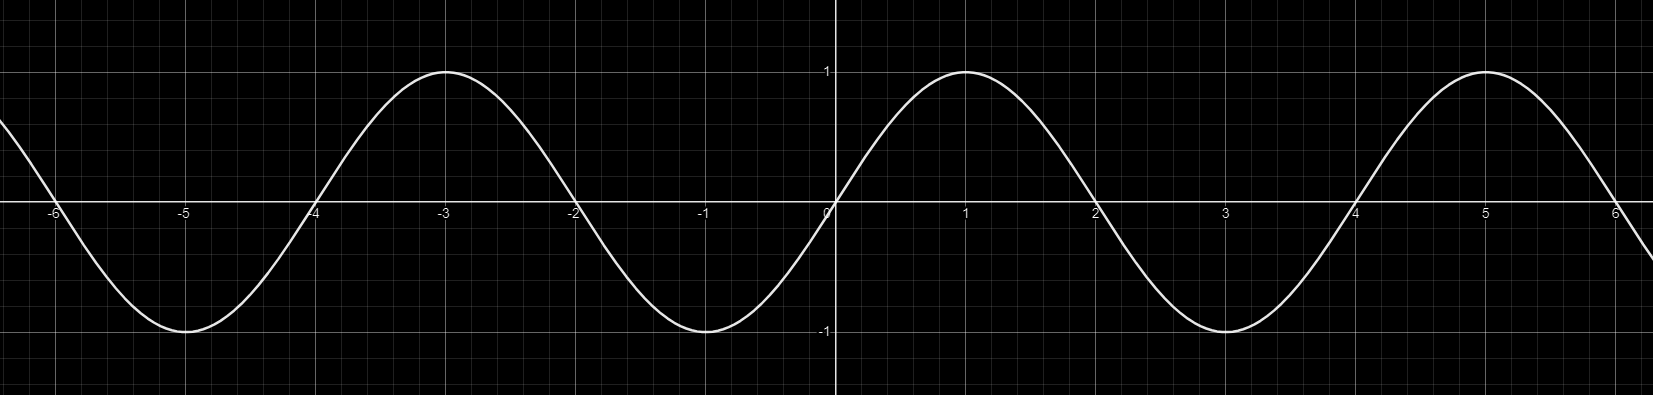
\includegraphics[scale=0.305]{graphs/2D_Real_New/FigureA}
\end{align*}
\hspace{21mm}\caption{Figure 1: Plot of $f_2(x)$ without scaling coefficients on the interval $-6 < x < 6$}

\begin{align*}
  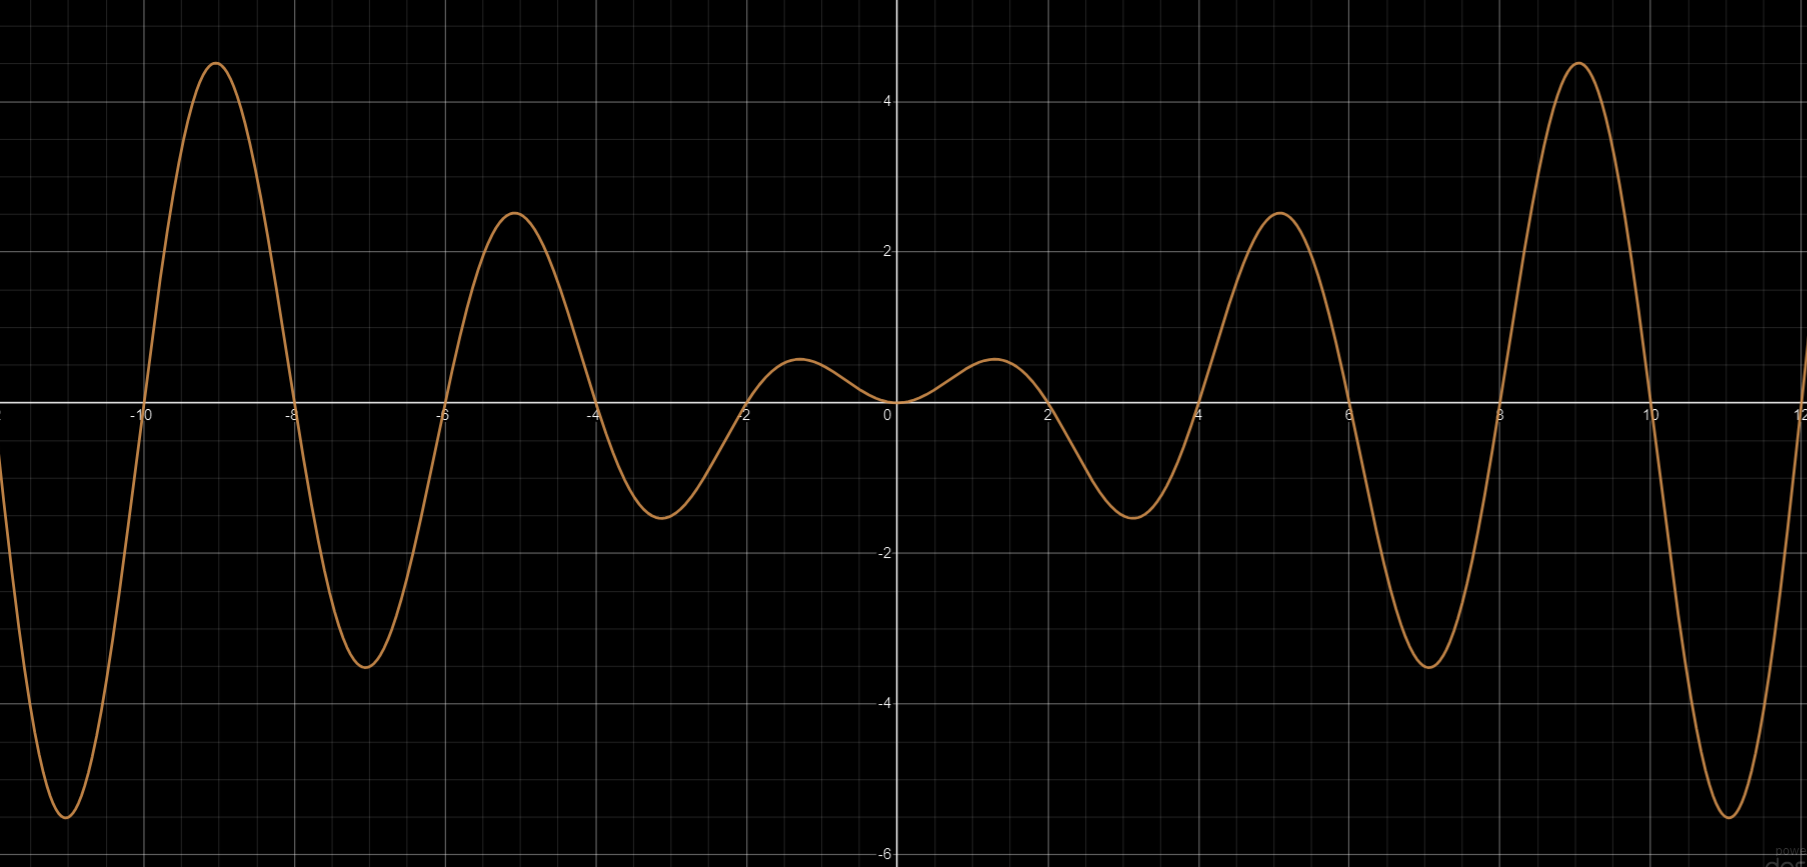
\includegraphics[scale=0.28]{graphs/2D_Real_New/Figure1_2}
\end{align*}
\hspace{21mm}\caption{Figure 2: Plot of $f_2(x)$ with scaling coefficients on the interval $-13 < x < 13$}

The two desired properties of an $a_k(x)$ function are (1) its amplitude is equal to $\alpha \frac{x}{k}$ and (2) its zeros are integer multiples of k.
Now, iterating this process, we will create an $a_k(x)$ for each whole number like so:

\begin{align*}
	a_2(x) = |\alpha \frac{x}{2}\sin\left(\frac{\pi x}{2}\right)| \\
	a_3(x) = |\alpha \frac{x}{3}\sin\left(\frac{\pi x}{3}\right)| \\
	a_4(x) = |\alpha \frac{x}{4}\sin\left(\frac{\pi x}{4}\right)|	\\
	a_5(x) = |\alpha \frac{x}{5}\sin\left(\frac{\pi x}{5}\right)| \\
	a_6(x) = |\alpha \frac{x}{6}\sin\left(\frac{\pi x}{6}\right)|	\\
	...
\end{align*}

Now plotting an $a_k(x)$ function for every whole number, except for 1, whose graph is shown without scaling coefficients in Figure 3, and with scaling coefficients in Figure 4.

\begin{align*}
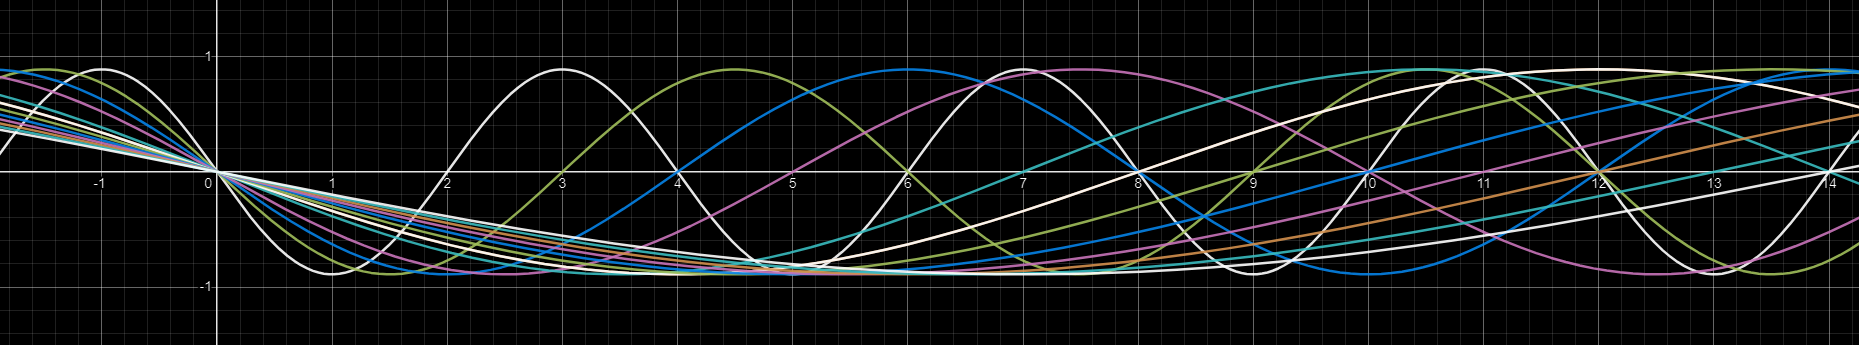
\includegraphics[scale=0.31]{graphs/2D_Real_New/FigureB_redone}
\end{align*}
\hspace{15mm}\caption{Figure 3: Graph of the Sieve of Eratosthenes, without Scaling}

\begin{align*}
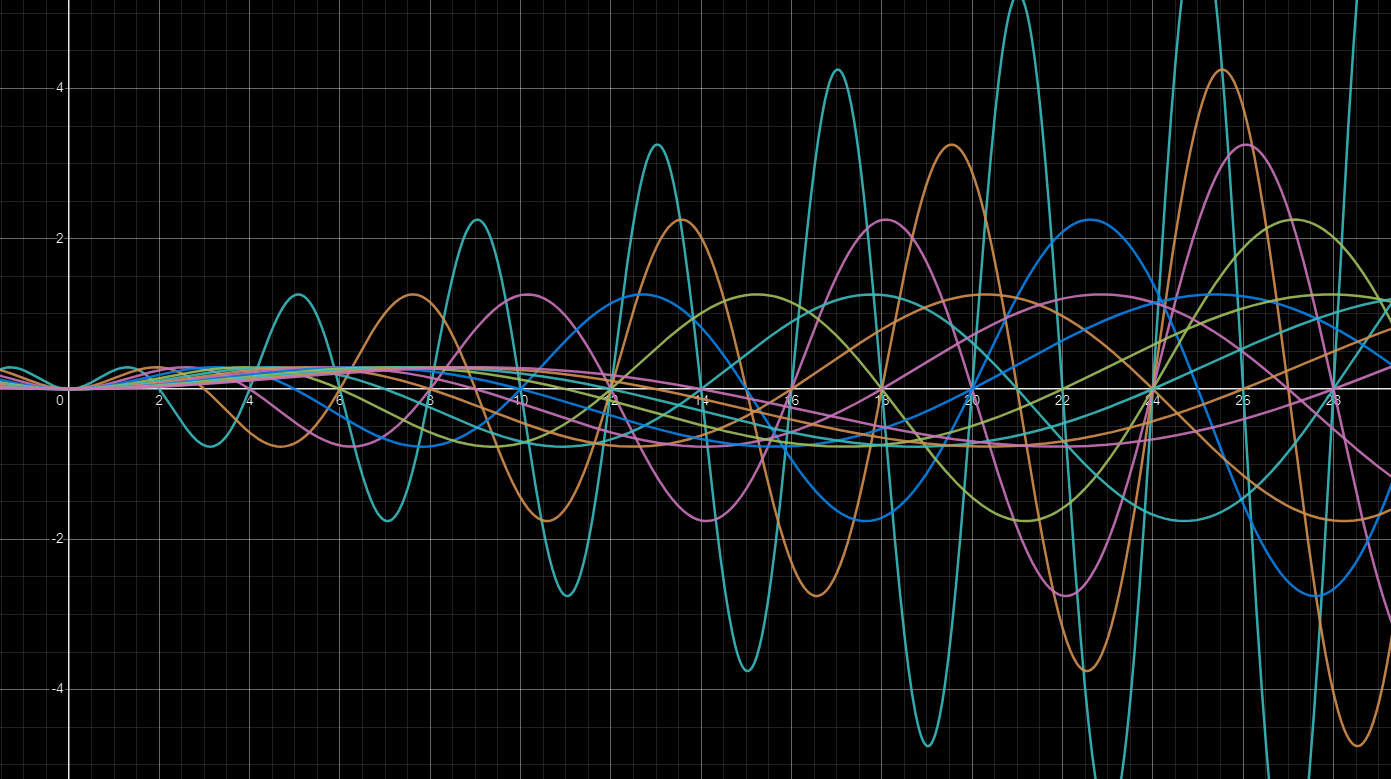
\includegraphics[scale=0.33]{graphs/2D_Real_New/Figure4_redone}
\end{align*}
\hspace{15mm}\caption{Figure 4: Graph of the Sieve of Eratosthenes, with Scaling} \\

By doing this, we have essentially created the Sieve of Eratosthenes using sine waves. You will notice that at each prime number there is only one $a_k(x)$ wave passing through the x axis. If we had created an $a_1(x)$ function then there would be 2 $a_k(x)$ waves passing through each prime x-intercept. “A prime is only divisible by itself, and one.” Because we reject $a_1(x)$ and go straight to $a_2(x)$, this means the wave passing through any prime x-intercept is the $a_p(x)$ where P is that prime number. I.e., $a_2(x)$, $a_3(x)$, $a_5(x)$, $a_7(x)$, $a_1_1(x)$, $a_1_3(x)$, etc. \\
\newline
Now that we have created an infinite number of waves, each representing a different possible divisor, we can combine them into one wave function which has attributes from each divisor wave. We do this by using an Infinite Product to define our set of infinitely many waves. Refer to the function a(z) in the next section.

\subsection*{II. Initial Description of Function a(z)}
In this paper, we will analyze several special functions using divisor waves and extreme operators. Specifically, we will consider the functions $a(z)$, $b(z)$, $c(z)$, $d(z)$, $e(z)$, $f(z)$, $g(z)$, $h(z)$, $i(z)$, $j(z)$, $k(z)$, $l(z)$, $m(z)$, $n(z)$, $o(z)$, and the Riemann zeta function $\zeta(z)$. These functions are of the variable z, where $z = x + iy$, this will be important as sometimes the scaling coefficients will be changed from x, to iy, to $x*iy$, to $x + iy$, to explore many domains/dimensions. \\

We define the function $a(z)$ as follows:

\begin{align*}
	a(z) = |\prod_{k=2}^x \alpha\frac{x}{k}\sin\left(\frac{\pi z}{k}\right)|
\end{align*}
	
The Function a(z) is the infinite product of $sin(\pi*z/k)$ where $2 <= k <= x$. This function, is part of a family of functions, that provide a map of the prime, and composite numbers. The front term $\alpha\frac{x}{k}$ is used for scaling purposes, as this function is highly explosive in the y-direction as you move down the x-axis. The alpha is just a coefficient that has a slider ranging from $0<\alpha<2$ and is used to stretch the function as needed. \\
\newline
The absolute value operator in front ensures that this function stays above the x-axis. This has the same effect as $y=abs[sin(x)]$. On the inside of the sine function, we still have the $\pi$ coefficient but have now replaced the whole number associated with the $f_k(z)$ function with k so that we can test through an infinite number of whole numbers.
\begin{align*}
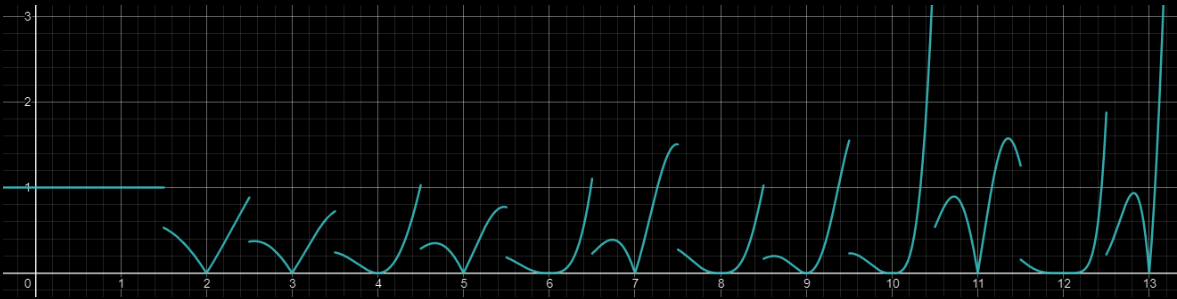
\includegraphics[scale=0.5]{graphs/2D_Real_Graphs/cuspcurve}
\end{align*}
\hspace{8mm}\caption{Figure 5: Real plot for a(x), on the interval $0 < x < 13$} \\

The Function a(x) is the infinite product of sinusoidal Divisor Waves, this essentially combines them all into one resultant wave. Looking at the graph, you can see that at each prime number there is a cusp, and at each composite number there is a curve. This is a result of the way the function approaches zero at that point. This Concept will apply to the proceeding functions as well and will allow us to analyze the continuity at each point and extract meaningful information. \\
\newline
COMPOSITE - At each composite number there are many waves all being combined at one point. For composite numbers there are more Divisor Waves that have x-intercepts causing them to trend towards zero sooner. It is because of this that a curve is created. This is even more true for highly composite numbers as highly composite numbers contain more factors. See 12 for an example of highly composite. \\
\newline
PRIME - Prime numbers do not approach zero the same way. For a prime number, there are also many waves combining at one point, but only $a_p(x)$ has an x-intercept. This means that they only reach zero for a moment before returning to larger values, and this creates the cusp.

\begin{align*}
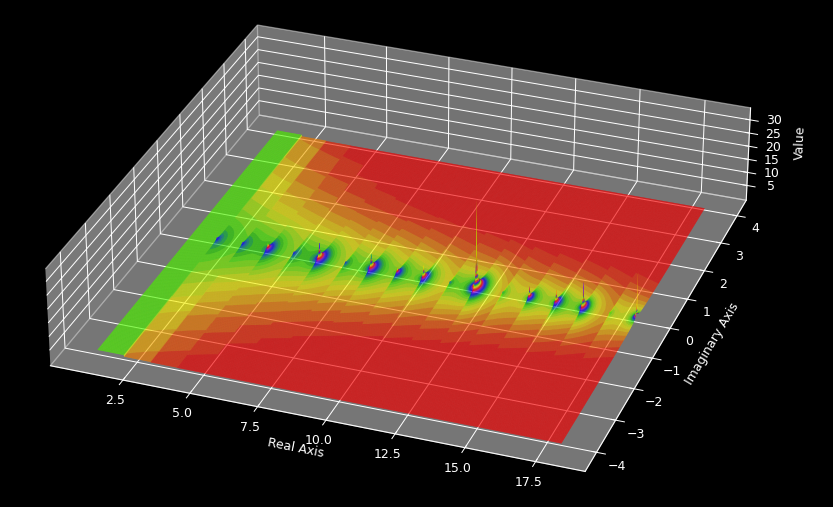
\includegraphics[scale=0.63]{graphs/3D_Complex_Graphs/product_of_sin/Complex_3D_product_of_sin_11}
\end{align*}
\hspace{15mm}\caption{Figure 6: 3D Graph of $a(x+iy)$ showcasing the zeros of the whole numbers in the complex domain on the interval of $1 < x < 18$} \\

The complex plot for a(z) reveals the same waveform with zeros at each of the whole numbers, however the composite numbers have far more distinguished peaks, as you gaze down the complex function you will see the distribution of zeros based on the distrtribution of prime and composite numbers, the peaks collecting at 8, 9, 10, 12, and 14 showcase this beautifully.
\begin{align*}
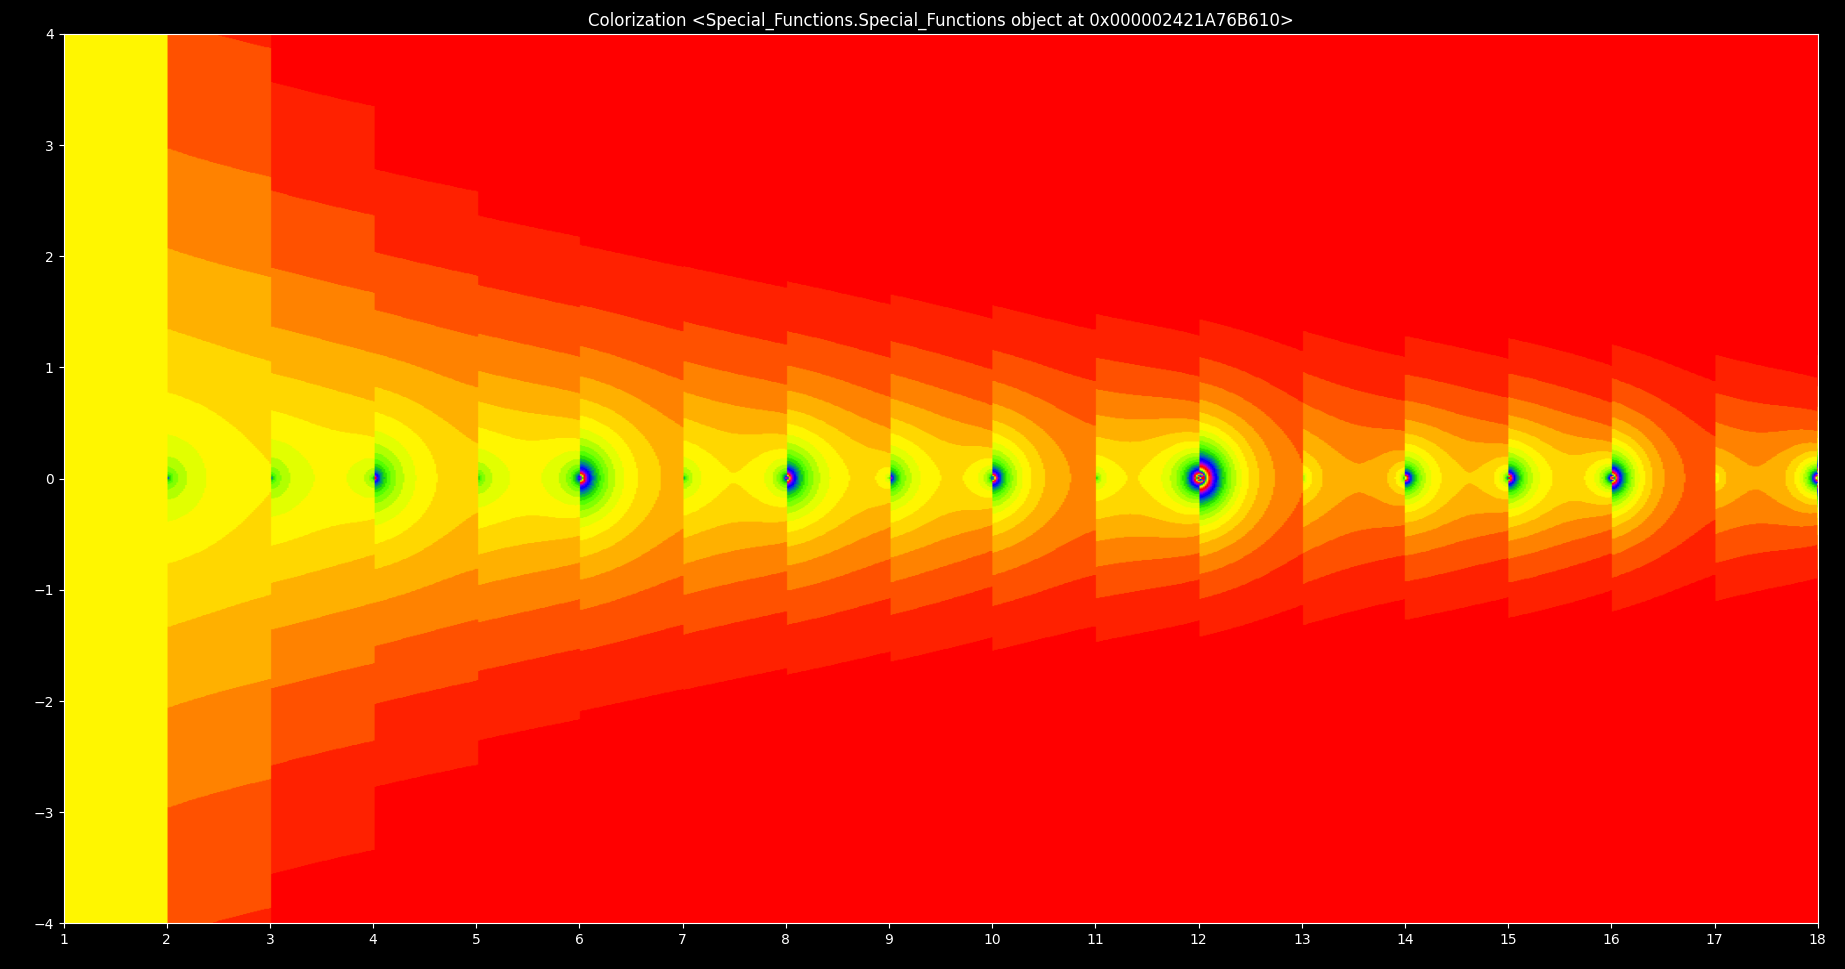
\includegraphics[scale=0.28]{graphs/3D_Complex_Graphs/product_of_sin/Complex_3D_product_of_sin_10}
\end{align*}
\hspace{8mm}\caption{Figure 7: 2D Graph of $a(x+iy)$ showcasing the zeros of the whole numbers in the complex domain on the interval of $1 < x < 18$} \\

\newpage
\subsection*{III. Initial Description of Function A(z)}
We define the Normalized a(z), function $A(z)$ as follows:
\begin{align*}
	A(z) = \frac{|\prod_{n=2}^x \alpha\frac{x}{n}\sin\left(\frac{\pi z}{n}\right)|^{-m}}{|\prod_{n=2}^x \alpha\frac{x}{n}\sin\left(\frac{\pi z}{n}\right)|^{-m}!}
\end{align*}
\begin{align*}
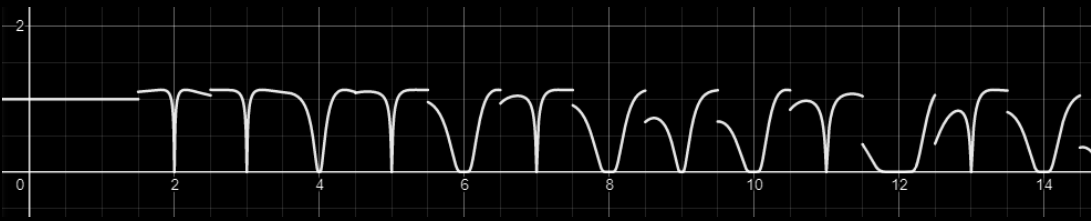
\includegraphics[scale=0.55]{graphs/2D_Real_Graphs/norm_cuspcurve}
\end{align*}
\hspace{8mm}\caption{Figure 8: 2D Graph of $A(x)$ showcasing the zeros of the real numbers} \\

This process is similar to linearization. By taking the original function a(z) and taking the fraction:
\begin{align*}
a(z)^{-m}/(a(z)^{-m})!
\end{align*} 

We are utilizing the factorial function to remove the explosive nature of a(z) and the exponent -m is a coefficient on a slider. This coefficient will allow us to magnify the function similar to $\alpha$. This actually stems from the following summation although this normalization utilizes infinite products:
\begin{align*}
\sum_{x=1}^\infty (\frac{x}{x!}) = e \rightarrow \prod_{x=1}^\infty (\frac{x}{x!}) = e^x
\end{align*}

\begin{align*}
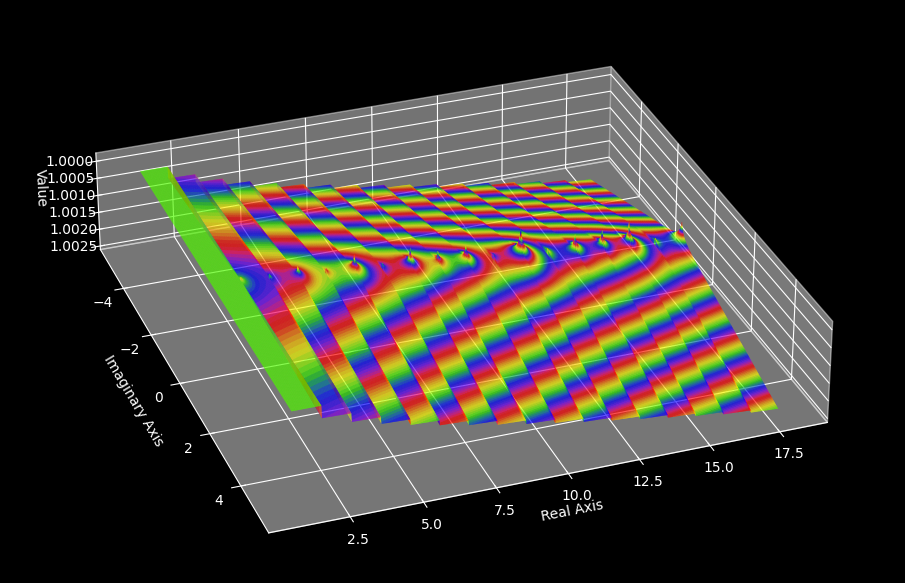
\includegraphics[scale=0.54]{graphs/3D_Complex_Graphs/product_of_sin/normalized_Complex_3D_product_of_sin_HDSET_5}
\end{align*}
\hspace{8mm}\caption{Figure 9: 3D Graph of $A(x+iy)$ showcasing the normalized zeros of the real numbers in the complex plane} \\

Similarly to Figure 6, Figure 9 showcases the complex plot for A(z) which is the normalized plot of a(z) and reveals the same waveform with zeros at each of the whole numbers, however the composite numbers have far more distinguished peaks, as you gaze down the complex function you will see the distribution of zeros based on the distribution of prime and composite numbers, the peaks collecting at 8, 9, 10, 12, and 14 showcase this beautifully.

\begin{align*}
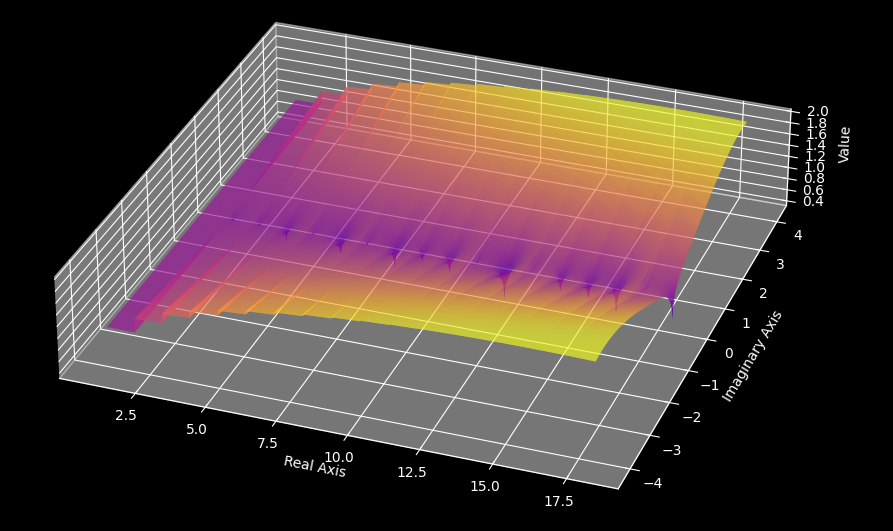
\includegraphics[scale=0.54]{graphs/3D_Complex_Graphs/product_of_sin/normalized_Complex_3D_product_of_sin_HDSET_4}
\end{align*}
\hspace{8mm}\caption{Figure 10: 3D Graph of $A(x+iy)$ showcasing the normalized zeros of the real numbers in the complex plane} \\

As you can see from the complex plots, A(z) is a function with zeros at all real numbers greater than 1, and for composite numbers contains many divisor waves which create larger peaks, or dips.

\begin{align*}
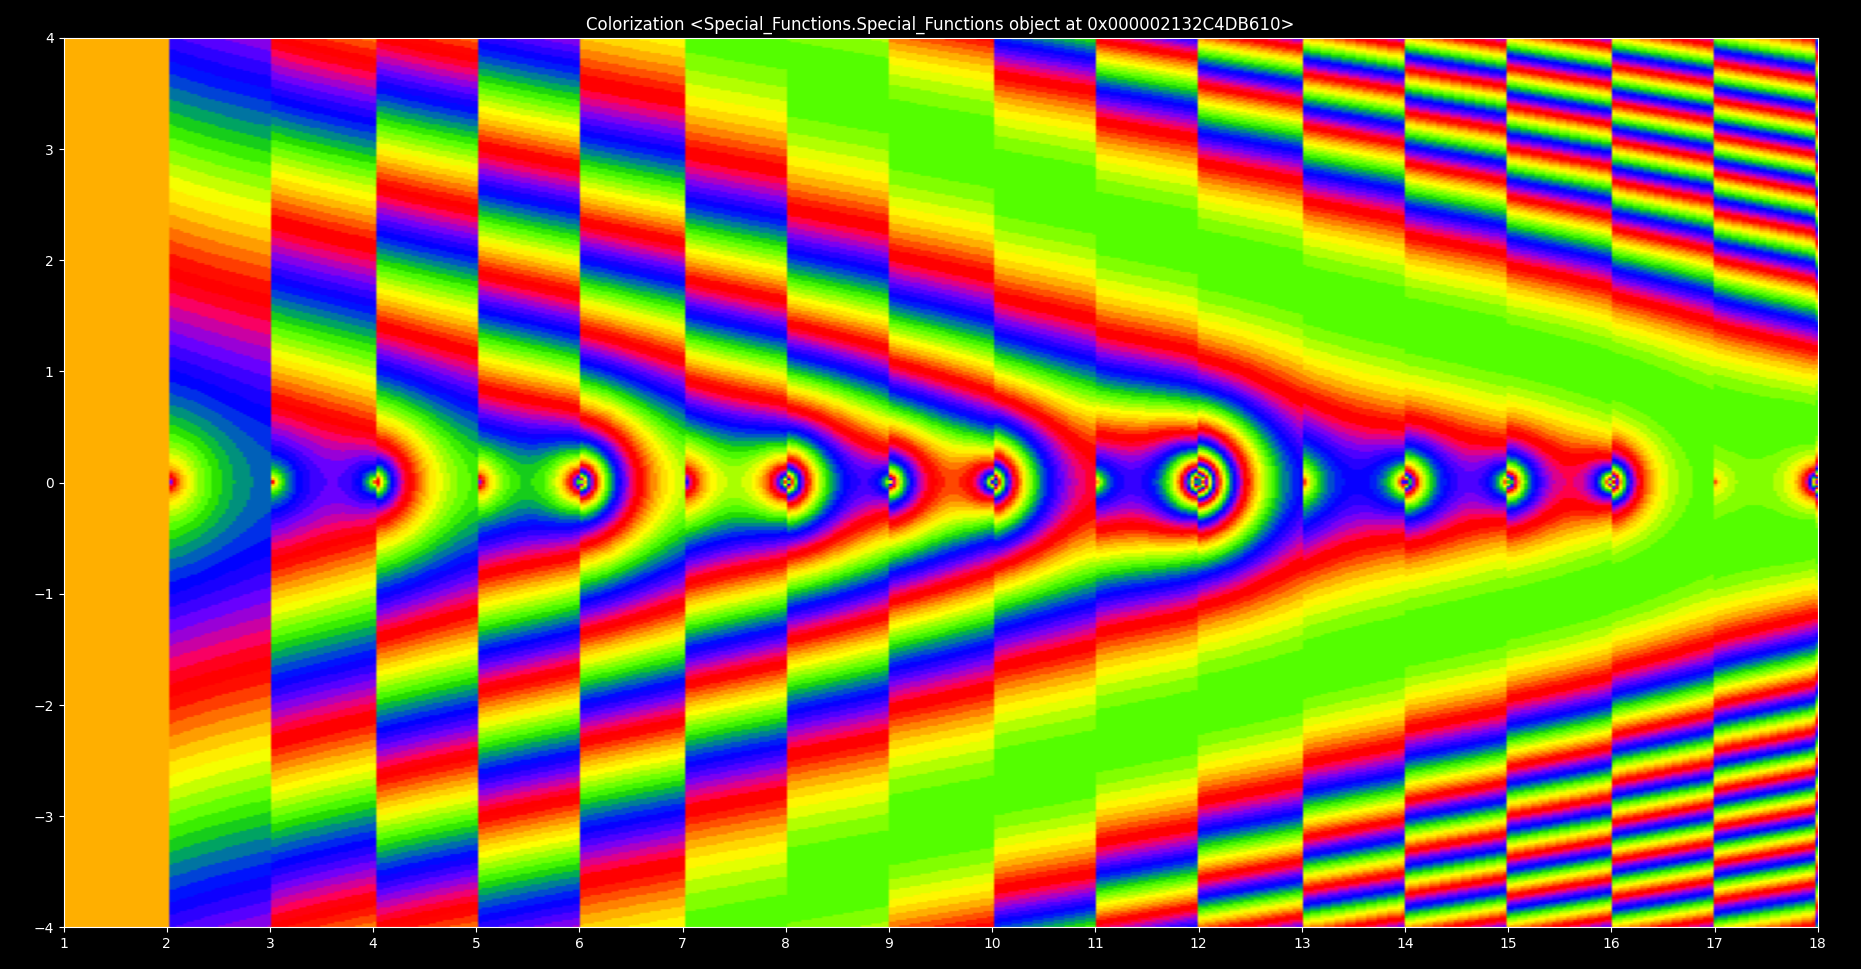
\includegraphics[scale=0.28]{graphs/3D_Complex_Graphs/product_of_sin/normalized_Complex_3D_product_of_sin_HDSET_8}
\end{align*}
\hspace{8mm}\caption{Figure 11: 2D Graph of $A(x+iy)$ showcasing the normalized zeros of the real numbers in the complex plane} \\

\newpage
\subsection*{IV. Initial Description of Function b(z)}
The function $b(z)$ is defined as the infinite product of the infinite product representation of $\sin(\pi*z/n)$:
\begin{align*}
	b(z) = |\prod_{k=2}^x \left[\frac{\beta x}{k}\left({\pi z}\prod_{n=2}^x\left(1 - \frac{z^2}{n^2k^2}\right)\right)\right]|
\end{align*}
\begin{align*}
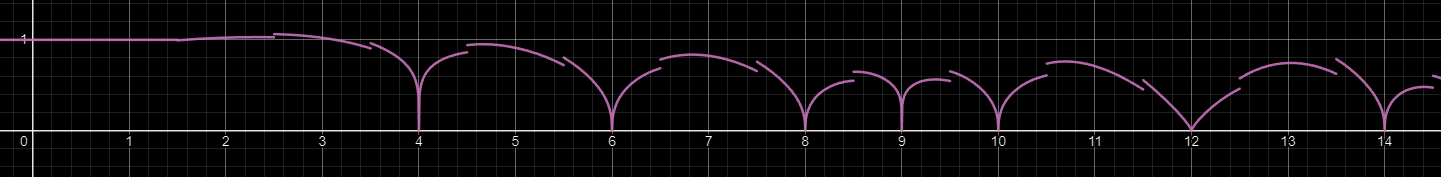
\includegraphics[scale=0.45]{graphs/2D_Real_Graphs/prime_indicator_og_redone}
\end{align*}
\hspace{8mm}\caption{Figure 12: 2D Graph of $b(x)$ showcasing the zeros of the composite numbers} \\

The Function b(x) is the infinite product of the modified product representation for sin, this essentially combines all of these modified sin waves into one resultant wave. Looking at the graph, you can see that at each prime number there is a curve, and at each composite number there is a cusp. \\
\newline
COMPOSITE - At each composite number there are many waves all being combined at one point. For composite numbers there are Divisor Waves that have x-intercepts, and in the range of primes contain no Divisor Waves going to zero, so the boundary from composite to prime causes them to trend towards zero. It is because of this that a cusp is created. Highly Composite numbers in this context actually have less of a cusp due to having more factors. See 12 for an example of highly composite. \\
\newline
PRIME - Prime numbers do not approach zero at all in this case. For a prime number, there are also many waves combining at one point, but only $b_p(x)$ has an x-intercept, and since we modified the index to be n=2 we reject the zeros with a factor of 1. This means that they never reach zero in the domain of a prime number, and this creates the non-zero curve.
\begin{align*}
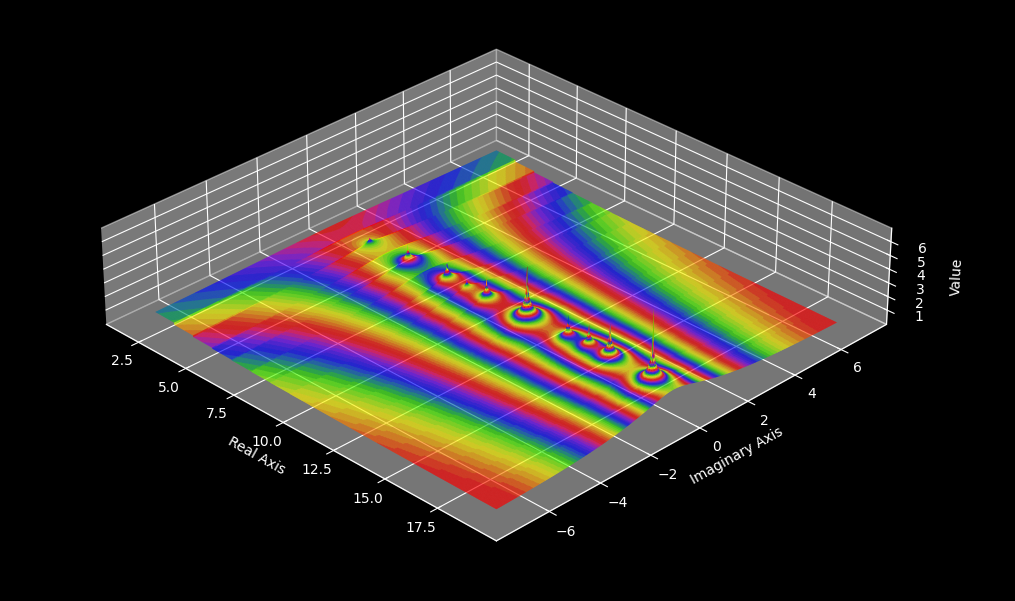
\includegraphics[scale=0.45]{graphs/3D_Complex_Graphs/product_of_product_representation_of_sin/non_normalized_goodm_prism_1}
\end{align*}
\hspace{8mm}\caption{Figure 13: 2D Graph of $b(x+iy)$ showcasing the zeros of the composite numbers} \\

We can see the zeros of $b(x + iy)$ as the blue troughs in the hills. These are the composite numbers. For each composite number there is a factor causing the product to go to zero. For all whole number values of x where x is prime, the function does not go to zero. We can observe this phenomenon at 11, and 13 on the graph as these are prime numbers. \\
\begin{align*}
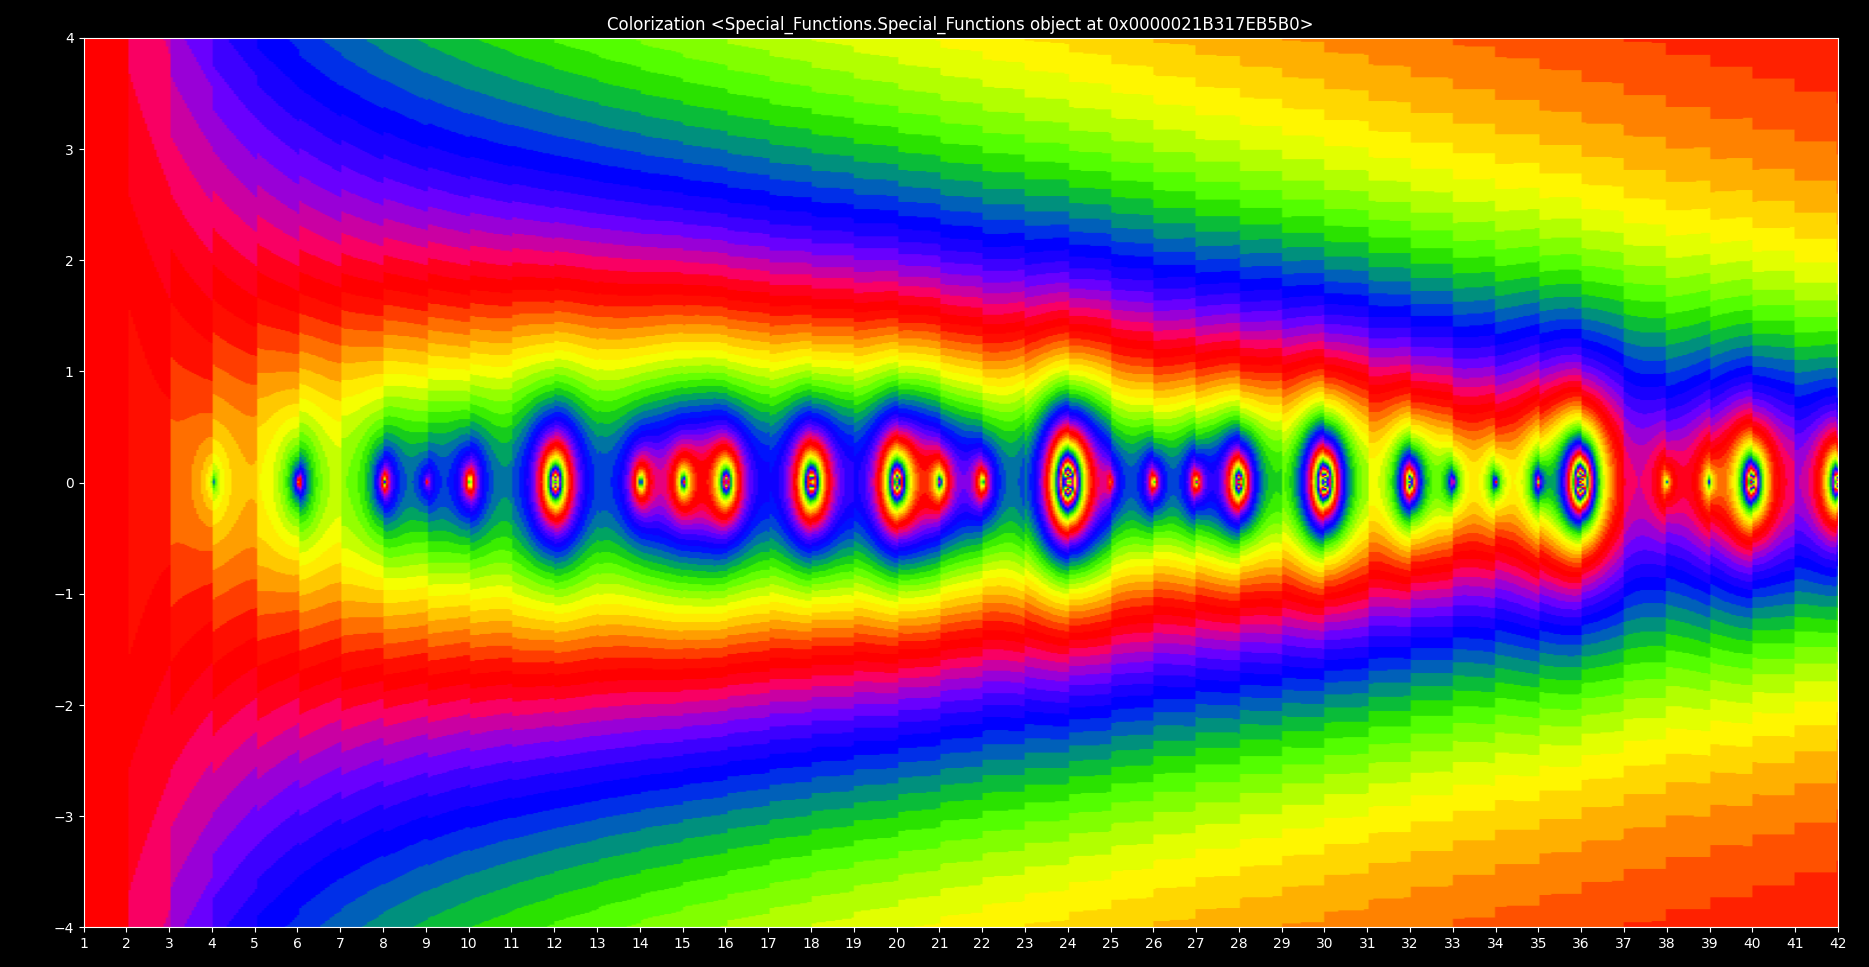
\includegraphics[scale=0.28]{graphs/3D_Complex_Graphs/product_of_product_representation_of_sin/non_normalized_goodm_prism_8}
\end{align*}
\hspace{8mm}\caption{Figure 14: 3D Graph of $b(x+iy)$ showcasing the zeros of the composite numbers} \\

The above graph is the 3D plot for $b(x+iy)$ where the 3rd dimension is height. This graph shows the complexity of the primes as it is solely dependant on the distribution of composite numbers. \\

\begin{align*}
\includegraphics[scale=0.28]{graphs/2D_Complex_Graphs/Infinite_Product_of_infinite_product_representation_of_sin/Complex_product_17_n_2-28__imaginary_scalar_logarithm}
\end{align*}
\hspace{8mm}\caption{Figure 15: 2D Fractal $#2$ Graph of $b(x+iy)$ showcasing the zeros of the composite numbers by Multipling $b(x+iy) * iy$} \\

The above fractal is the graph of b(x+iy) * iy this multiplies the function by the imaginary component which allows the values to stetch away from the $x-axis$ providing a beautiful fractal for the prime and composite numbers. The spikes are locations with many factors, the factors cause the function to go to infinity in the complex dimension. The prime numbers can be seen as curves between the cusps. These curves are the result of having less component waves that go to zero. \\

\newpage
Derivation of b(z) by substituting the infinite product representation of $sin(\pi*z/n)$ into the infinite product of $\sin(\pi*z/n)$: \\

Starting with function a(z): \\
\begin{align*}
	a(z) = |\prod_{k=2}^z \alpha\frac{z}{k}\sin\left(\frac{\pi z}{k}\right)| \\
\end{align*}

We use the Weierstrass Product Formula for sin to form the relationship where k is a constant: \\
\begin{align*}
	\sin\left(\frac{\pi z}{k}\right) = \pi z\prod_{n=2}^z \left(1-\frac{z^2}{n^2k^2}\right) \\
\end{align*}

Taking the product of both sides we have the functional equation of a(z) known as b(z): \\
\begin{align*}
	\prod_{k=2}^z\sin\left(\frac{\pi z}{k}\right) = \prod_{k=2}^z \pi z\prod_{n=2}^z \left(1-\frac{z^2}{n^2k^2}\right) \\
\end{align*}

This proof shows the relationship between a(z) and b(z), and allows us to appreciate some of the beautiful relationships between these functions. The function b(z) is an equivalent form of a(z) however it has extra parameters that we can use to our advantage. \\

Now, we can expand the product out to infinity, using the expression we derived earlier:

\begin{align*}
f(x) &= \prod_{k=2}^{x} \left|\frac{\pi x}{k} \prod_{n=2}^{\infty} \left( 1 - \frac{x^2}{n^2 k^2} \right) \right| \\
&= \prod_{k=2}^{x} \left|\frac{\pi x}{k} \prod_{n=2}^{\infty} \left( 1 - \frac{x^2}{n^2 k^2} \right) \right| \\
&= \prod_{k=2}^{x} \left|\frac{\pi x}{k} \left[ \left( 1 - \frac{x^2}{(2^2)(k^2)}\right) \left( 1 - \frac{x^2}{(3^2)(k^2)}\right) \left( 1 - \frac{x^2}{(4^2)(k^2)}\right) \cdots \right]\right| \\
\end{align*}
\begin{align*}
&= \frac{\pi*x}{n}\left[ \left( 1 - \frac{x^2}{(2^2)(2^2)}\right) \left( 1 - \frac{x^2}{(2^2)(3^2)}\right) \left( 1 - \frac{x^2}{(2^2)(4^2)}\right) \cdots \right] \\
&\qquad \times \left[ \left( 1 - \frac{x^2}{(3^2)(2^2)}\right) \left( 1 - \frac{x^2}{(3^2)(3^2)}\right) \left( 1 - \frac{x^2}{(3^2)(4^2)}\right) \cdots \right] \\
&\qquad \times \left[ \left( 1 - \frac{x^2}{(4^2)(2^2)}\right) \left( 1 - \frac{x^2}{(4^2)(3^2)}\right) \left( 1 - \frac{x^2}{(4^2)(4^2)}\right) \cdots \right] \\
&\qquad \times \cdots \\
\end{align*}

\newpage
We can now use this infinite polynomial to evaluate the composite number $x = 4$ and we can see that for the factors of 4 the terms of the polynomial go to zero. \\

\begin{flushleft*}
f(4) = \\
\end{flushleft*}

\begin{align*}
= \pi*4\left\left[ \left( 1 - \frac{4^2}{(2^2)(2^2)}\right) \left( 1 - \frac{4^2}{(2^2)(3^2)}\right) \left( 1 - \frac{4^2}{(2^2)(4^2)}\right) \right] \\
\times \left[ \left( 1 - \frac{4^2}{(3^2)(2^2)}\right) \left( 1 - \frac{4^2}{(3^2)(3^2)}\right) \left( 1 - \frac{4^2}{(3^2)(4^2)}\right) \right] \\
\times \left[ \left( 1 - \frac{4^2}{(4^2)(2^2)}\right) \left( 1 - \frac{4^2}{(4^2)(3^2)}\right) \left( 1 - \frac{4^2}{(4^2)(4^2)}\right) \right] \\
= \pi*4\left\left[ \left( 1 - \frac{16}{(4)(4)}\right) \left( 1 - \frac{16}{(16)(9)}\right) \left( 1 - \frac{16}{(4)(16)}\right) \right] \\
\times \left[ \left( 1 - \frac{16}{(9)(4)}\right) \left( 1 - \frac{16}{(9)(9)}\right) \left( 1 - \frac{16}{(9)(16)}\right) \right] \\
\times \left[ \left( 1 - \frac{16}{(16)(4)}\right) \left( 1 - \frac{16}{(16)(9)}\right) \left( 1 - \frac{16}{(16)(16)}\right) \right] \\
= \cdots \left( 1 - \frac{4^2}{(2^2)(2^2)}\right) \cdots \\
= \left( 1 - \frac{4^2}{(4)(4)}\right) = 0 \\
\end{align*}

For completeness we will also evaluate the prime number $x = 3$ and we can see that for the factors of 3 none of the terms go to zero. \\

\begin{flushleft*}
f(3) = \\
\end{flushleft*}

\begin{align*}
= \pi*3\left\left[ \left( 1 - \frac{3^2}{(2^2)(2^2)}\right) \left( 1 - \frac{3^2}{(2^2)(3^2)}\right)  \right] \\
\times \left[ \left( 1 - \frac{3^2}{(3^2)(2^2)}\right) \left( 1 - \frac{3^2}{(3^2)(3^2)}\right)  \right] \\
= \pi*3\left\left[ \left( 1 - \frac{3^2}{(4)(4)}\right) \left( 1 - \frac{3^2}{(4)(9)}\right)  \right] \\
\times \left[ \left( 1 - \frac{3^2}{(9)(4)}\right) \left( 1 - \frac{3^2}{(9)(9)}\right)  \right] \\
= \pi*3\left\left[ \left( 1 - \frac{9}{(16)}\right) \left( 1 - \frac{9}{(36)}\right)  \right] \\
\times \left[ \left( 1 - \frac{9}{(36)}\right) \left( 1 - \frac{9}{(81)}\right)  \right] \\
= \pi*3\left\left[ \left(\frac{7}{(16)}\right) \left(\frac{27}{(36)}\right)  \right] \times \left[ \left(\frac{27}{(36)}\right) \left(\frac{72}{(81)}\right)  \right] \\
\end{align*}

\newpage
\subsection*{V. Initial Description of Function B(z)}
We define the Normalized b(z), function $B(z)$ as follows:

\begin{align*}
	B(z) = \frac{|\prod_{n=2}^x\left[\frac{\beta z}{n}\left({\pi z}\prod_{k=2}^z\left(1 - \frac{z^2}{k^2n^2}\right)\right)\right]|^{-m}}{|\prod_{n=2}^x\left[\frac{\beta z}{n}\left({\pi z}\prod_{k=2}^z\left(1 - \frac{z^2}{k^2n^2}\right)\right)\right]|^{-m}!}
\end{align*}

\begin{align*}
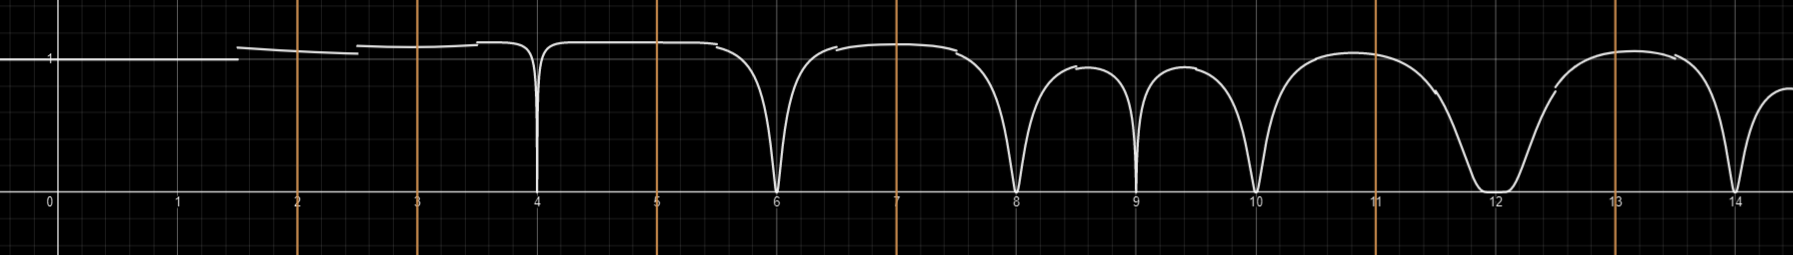
\includegraphics[scale=0.35]{graphs/2D_Real_Graphs/prime_indicator_norm}
\end{align*}
\hspace{8mm}\caption{Figure 16: 2D Graph of $B(x)$ showcasing the zeros of the composite numbers} \\

This Function is technically better than $A(z)$ as it allows us to control both of the index's n and k. By having access to n, we can have the initial value start at 2. This removes the divisor wave $B_1(x)$. Now the function no longer goes to zero at prime numbers and instead the function is greater than zero at primes and equal to zero at composites. \\

This Function is by far the most useful of the set as one could construct a piecewise function for $B(z)$ in which values of z are tested, if $B(z) > 0$, z is prime, if $B(z) = 0$, z is composite. \\

\begin{align*}
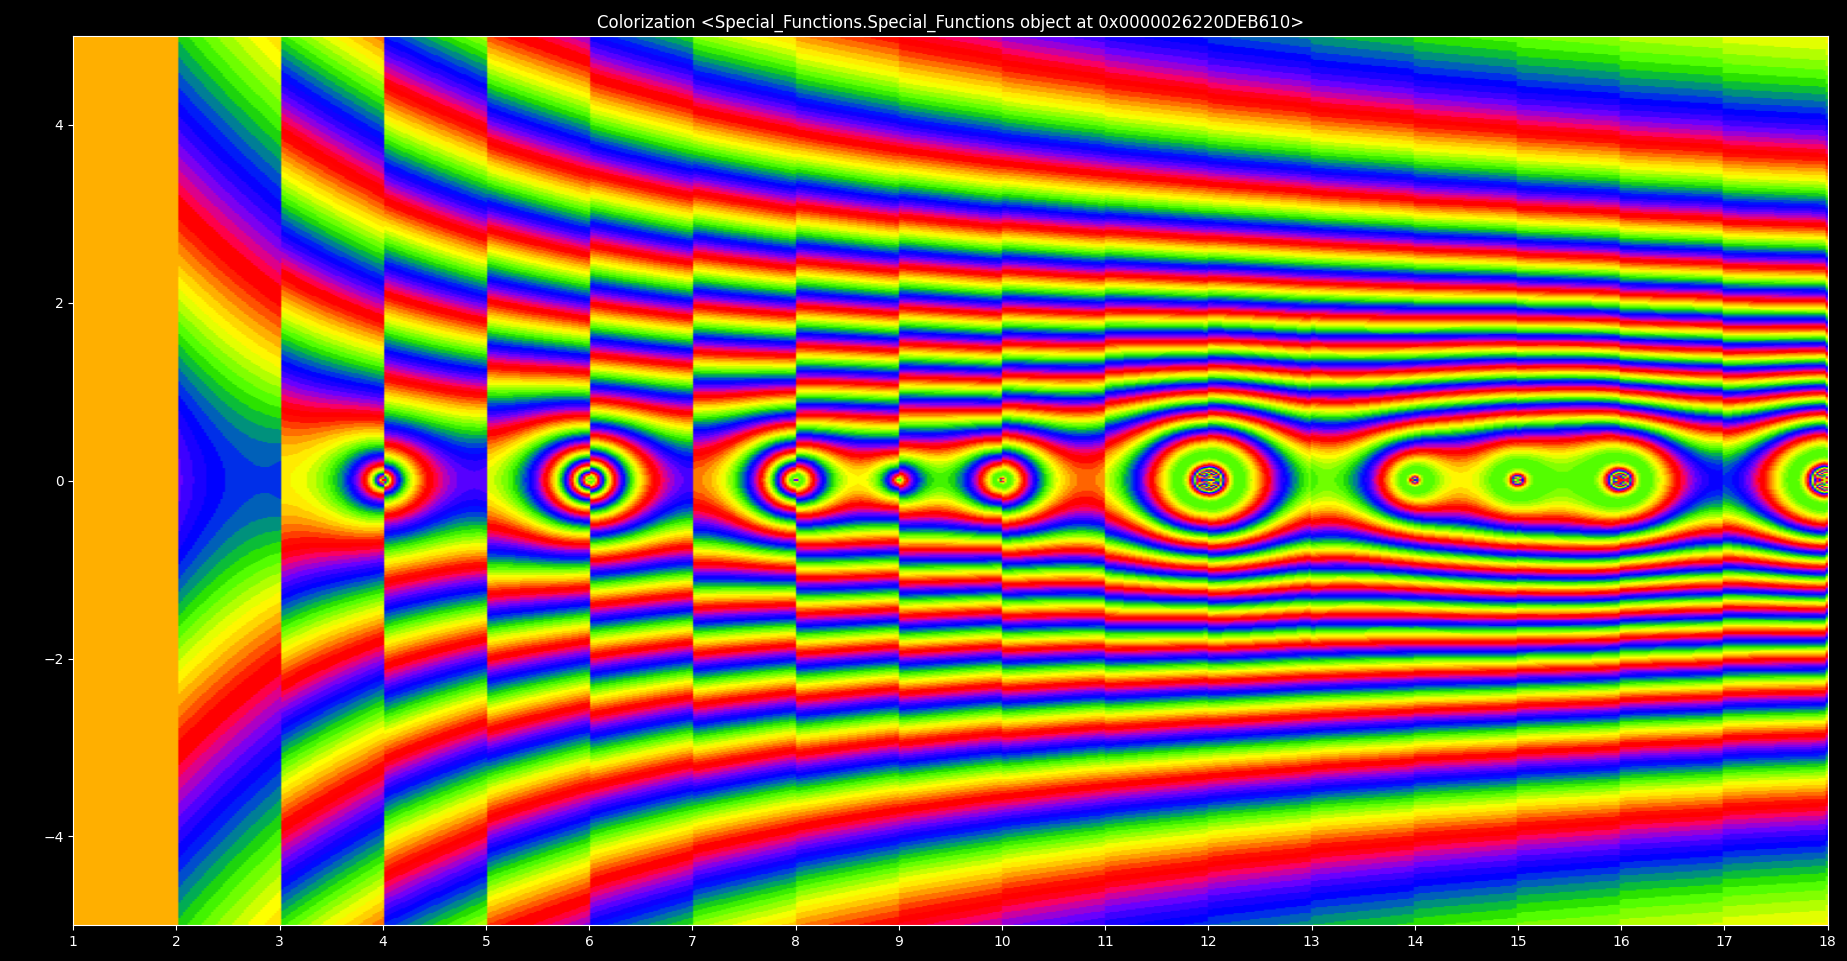
\includegraphics[scale=0.28]{graphs/3D_Complex_Graphs/product_of_product_representation_of_sin//ComplexPlot_prodprodforsin_4_Prism_Colorization_New}
\end{align*}
\hspace{8mm}\caption{Figure 17: 2D Graph of $B(x+iy)$ showcasing the zeros of the composite numbers} \\

The 2D plot of B(z) in the complex plane provides a map of the prime and composite numbers, the poles at composite numbers, versus the flat discontinuity at prime numbers show the relationship between the roots of B(z) and the composite numbers.

\begin{align*}
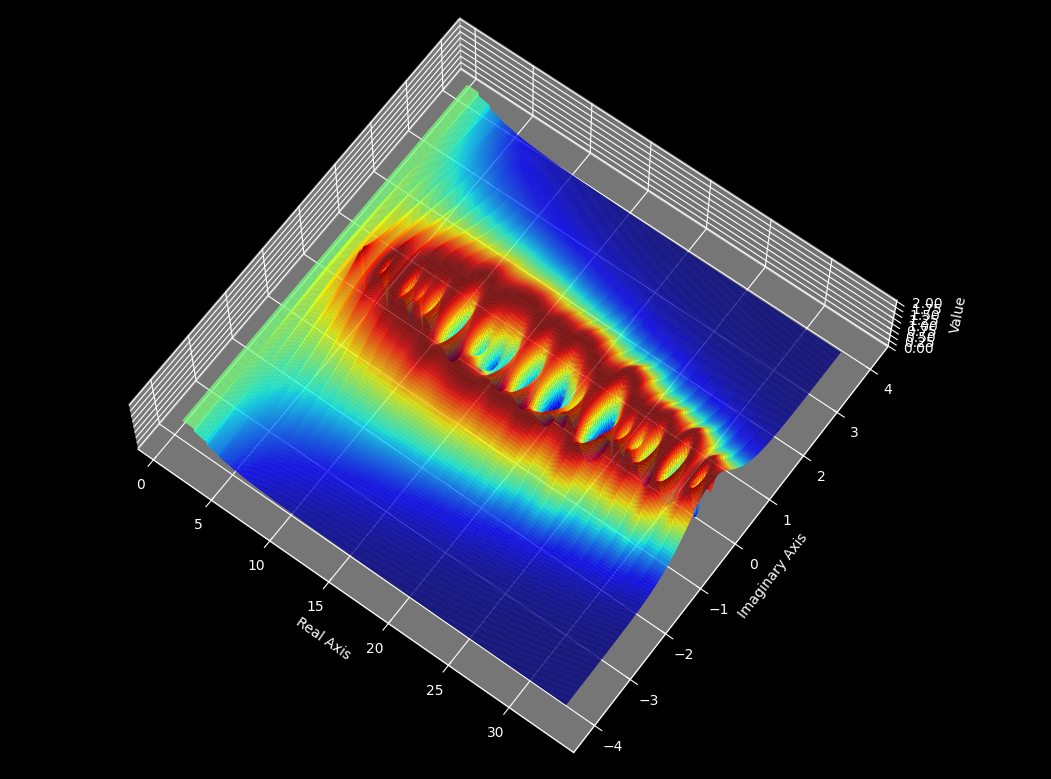
\includegraphics[scale=0.45]{graphs/3D_Complex_Graphs/product_of_product_representation_of_sin/ComplexPlot_prodprodforsin_8}
\end{align*}
\hspace{8mm}\caption{Figure 18: 3D Graph of $B(x+iy)$ showcasing the zeros of the composite numbers} \\

\begin{align*}
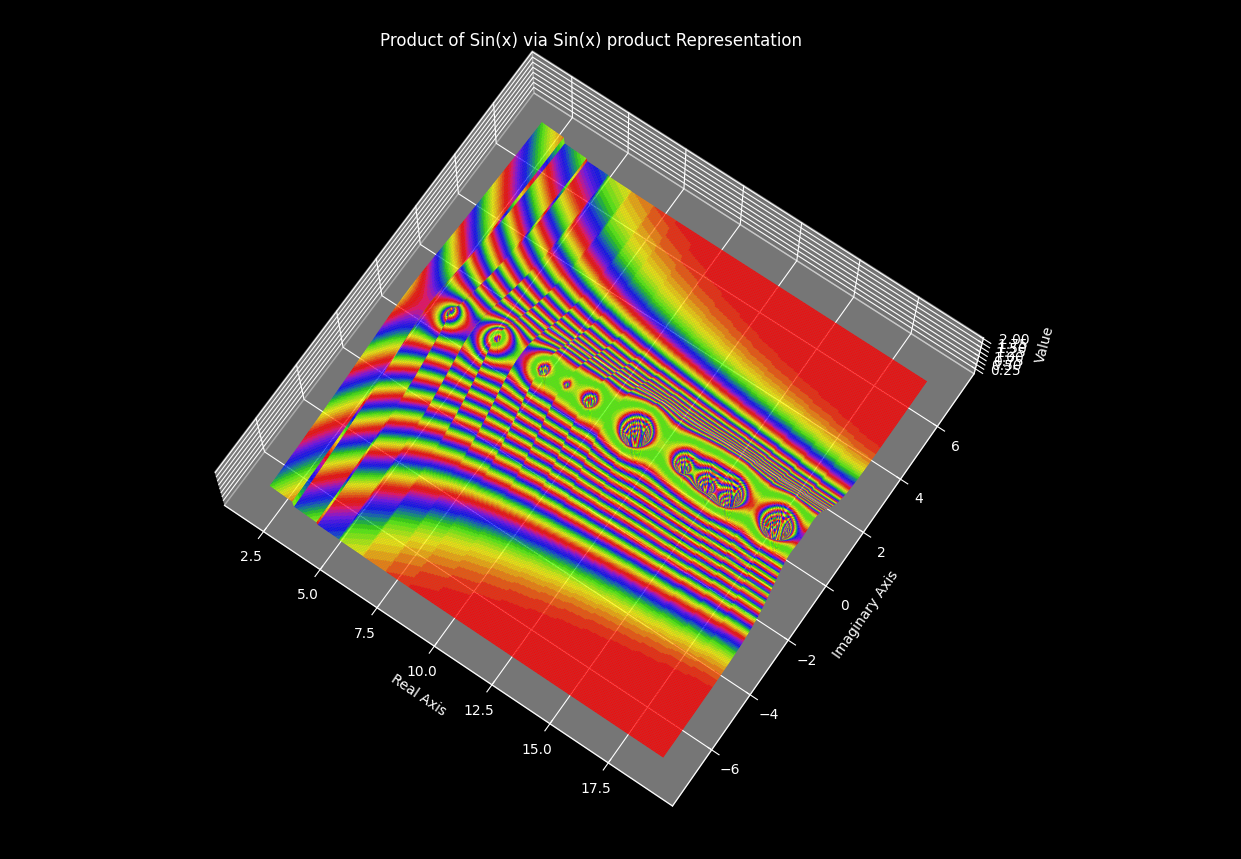
\includegraphics[scale=0.45]{graphs/3D_Complex_Graphs/product_of_product_representation_of_sin/ComplexPlot_norm_prodprodforsin_prism_3}
\end{align*}
\hspace{8mm}\caption{Figure 19: 3D Graph of $B(x+iy)$ showcasing the zeros of the composite numbers} \\

\newpage
\subsection*{Initial Description of Function g(z)}
The function $g(z)$ is defined as the infinite product of  of $1 + \sin(piz/n)$ and is a type of Riesz Product:

\begin{align*}
	g(z) = |\prod_{n=2}^z \left(1 + |\sin\left(\pi z n\right)|\right)|
\end{align*}

\newpage
\subsection*{Initial Description of Function G(z)}
We define the Normalized g(z), function $G(z)$ as follows:

\begin{align*}
	G(z) = \frac{|\prod_{n=2}^z \left(1 + |\sin\left(\pi z n\right)|\right)|^{-m}}{|\prod_{n=2}^z \left(1 + |\sin\left(\pi z n\right)|\right)|^{-m}!}
\end{align*} 

\begin{align*}
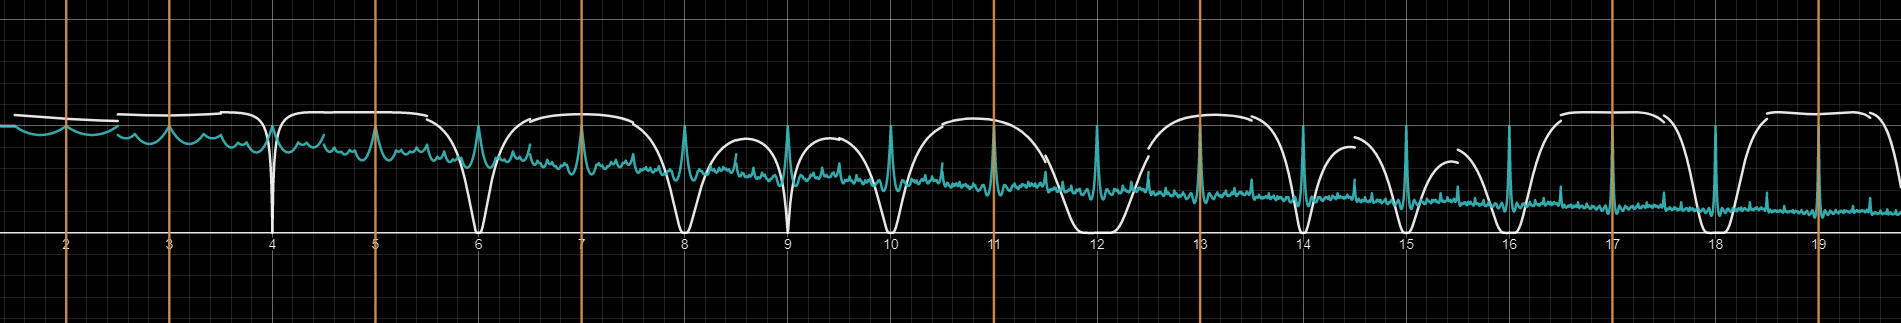
\includegraphics[scale=0.30]{graphs/2D_Real_Graphs/1+sin_prod}
\end{align*}

This function's waveform has peaks at each whole number value and smaller peaks between. This equation will be combined with b(z) later to create a waveform which is an indicator for prime and composite numbers while also dividing the space between whole numbers into finitely many sections as x goes to infinity.

\begin{align*}
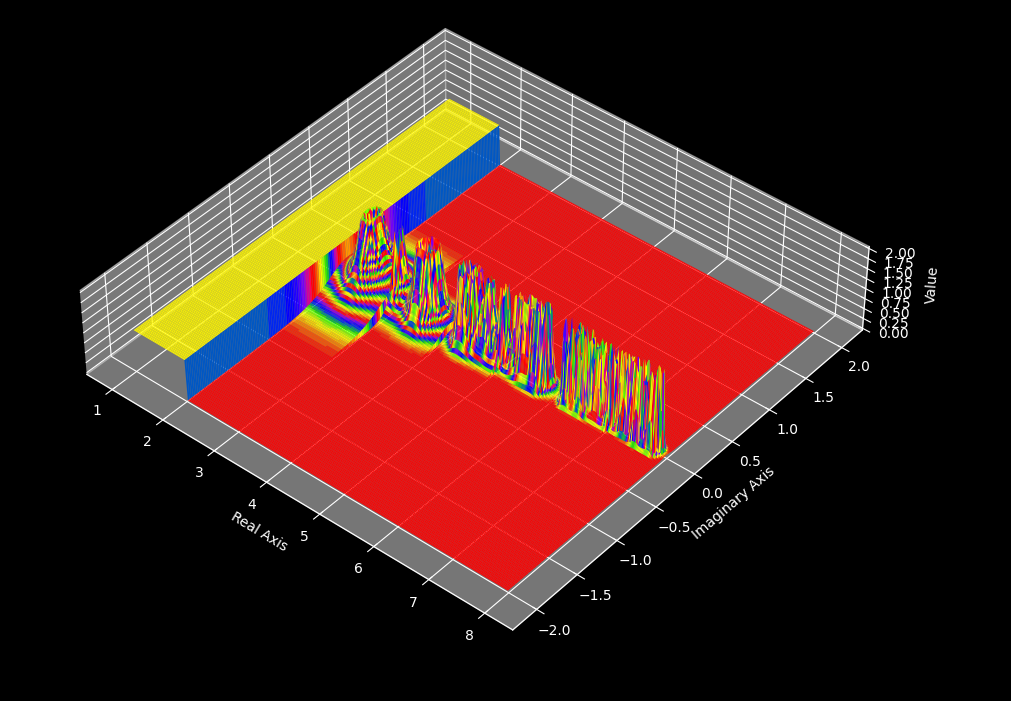
\includegraphics[scale=0.45]{graphs/3D_Complex_Graphs/riesz_sin/Ries_sin_norm_1}
\end{align*}

This is the normalized complex plot for Riesz' infinite product of sine. The plot is fascinating as it displays poles around specific values of x, similar to Riesz cosine product, and tangent product.

\newpage
\subsection*{Initial Description of Function h(z)}
The function $h(z)$ is defined as the infinite product of  of $1 + \cos(piz/n)$ and is a type of Riesz Product:

\begin{align*}
	h(z) = |\prod_{n=2}^z \left(1 + |\cos\left(\pi z n\right)|\right)|
\end{align*}

\newpage
\subsection*{Initial Description of Function H(z)}
We define the Normalized h(z), function $H(z)$ as follows:

\begin{align*}
	H(z) = \frac{|\prod_{n=2}^z \left(1 + |\cos\left(\pi z n\right)|\right)|^{-m}}{|\prod_{n=2}^z \left(1 + |\cos\left(\pi z n\right)|\right)|^{-m}!}
\end{align*} 

The second factor involves an infinite product of $(1 + cos(pixn))$ over all positive integers n between 2 and x. This is a way of constructing a product of terms that oscillate between positive and negative values, with the amplitude of the oscillation increasing as n increases. The factor of pi in the cosine function reflects the periodicity of the cosine wave.

Taken together, the two products combine to create a highly complex function that is difficult to analyze in general. However, it is clear that the function involves a combination of products of terms that are close to 1 and products of oscillating terms, which suggests that the function may exhibit highly irregular behavior as x varies. \\

\begin{align*}
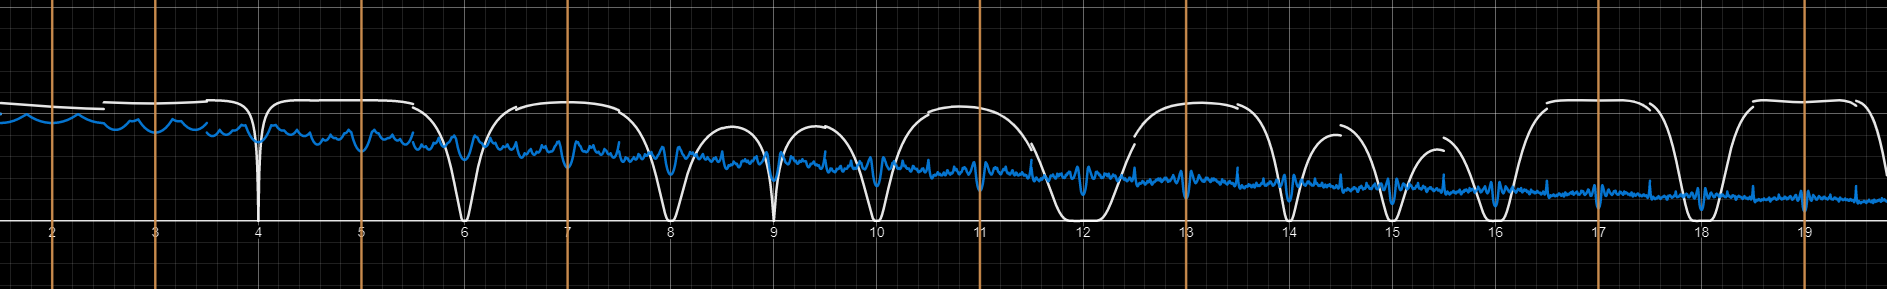
\includegraphics[scale=0.30]{graphs/2D_Real_Graphs/1+cos_prod}
\end{align*}

This function's waveform has troughs at each whole number value and smaller troughs between. This equation will be combined with b(z) later to create a waveform which is an indicator for prime and composite numbers while also dividing the space between whole numbers into finitely many sections as x goes to infinity.

\begin{align*}
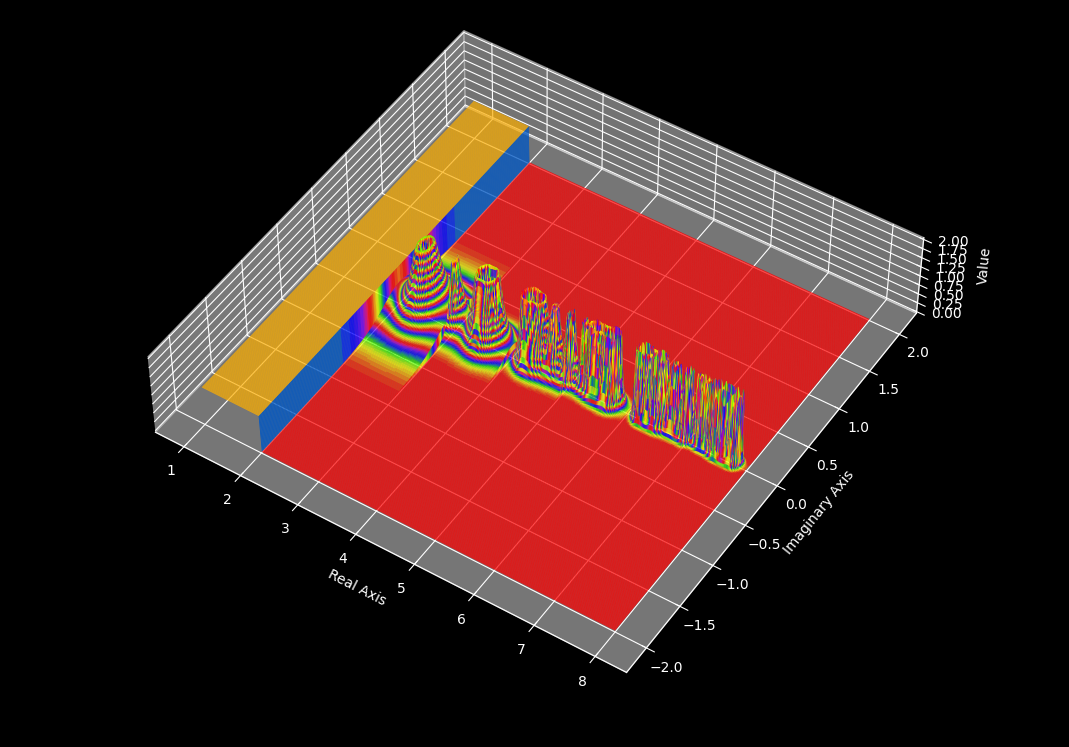
\includegraphics[scale=0.45]{graphs/3D_Complex_Graphs/riesz_cos/Ries_cos_norm_1}
\end{align*}

This is the normalized complex plot for Riesz' infinite product of cosine. The plot is fascinating as it displays poles around specific values of x, similar to Riesz sine product, and tangent product.

\newpage
\subsection*{Initial Description of Function i(z)}
The function $i(z)$ is defined as the infinite product of  of $1 + \tan(piz/n)$ and is a type of Riesz Product:

\begin{align*}
	i(z) = |\prod_{n=2}^z \left(1 + |\tan\left(\pi z n\right)|\right)|
\end{align*}

\newpage
\subsection*{Initial Description of Function I(z)}
We define the Normalized i(z), function $I(z)$ as follows:

\begin{align*}
	I(z) = \frac{|\prod_{n=2}^z \left(1 + |\tan\left(\pi z n\right)|\right)|^{-m}}{|\prod_{n=2}^z \left(1 + |\tan\left(\pi z n\right)|\right)|^{-m}!}
\end{align*} 

\begin{align*}
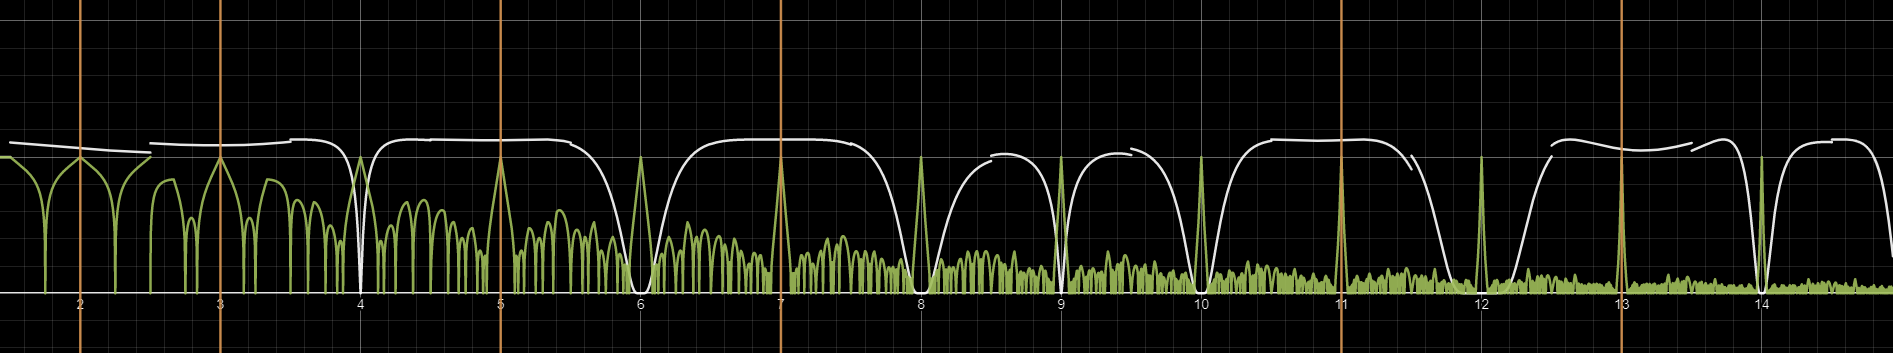
\includegraphics[scale=0.30]{graphs/2D_Real_Graphs/prod_1+tan}
\end{align*}

This function's waveform has peaks at each whole number value and bumpy patches between. These sections show nicely the divisions that are taking place accross the number line that section these areas into finitely many sections which increase as x goes to infinity. This equation will be combined with b(z) later to create a waveform which is an indicator for prime and composite numbers while also dividing the space between whole numbers into finitely many sections as x goes to infinity. \\

\begin{align*}
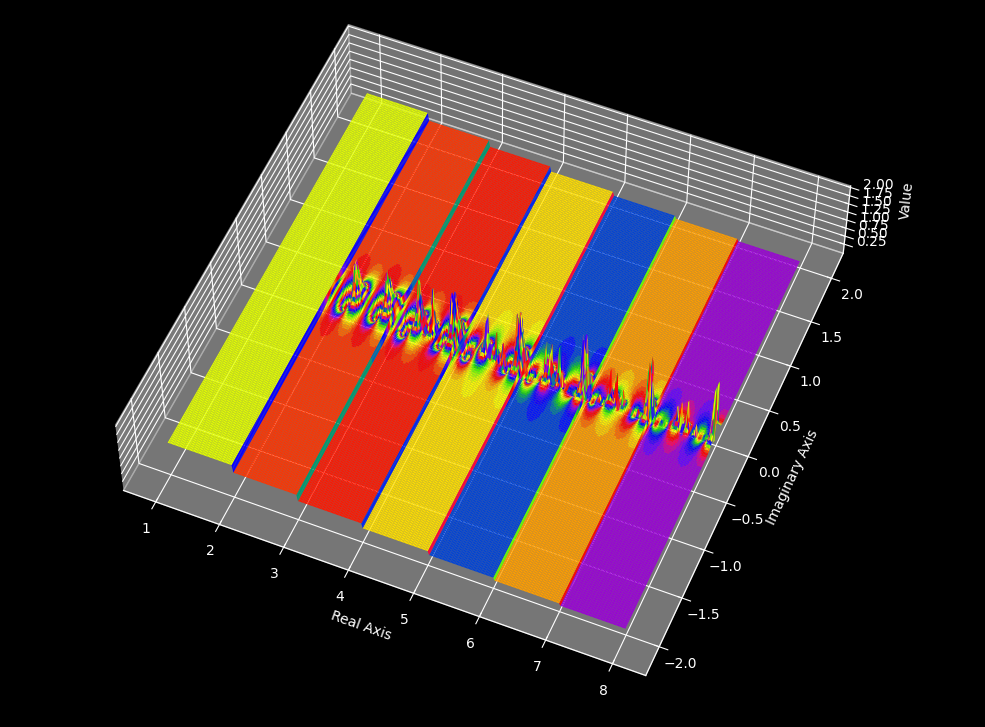
\includegraphics[scale=0.55]{graphs/3D_Complex_Graphs/riesz_tan/Ries_tan_norm_1}
\end{align*}

This is the normalized complex plot for Riesz' infinite product of tangent. The plot is fascinating as it displays poles around specific values of x, similar to Riesz sine product, and sine product.

\begin{align*}
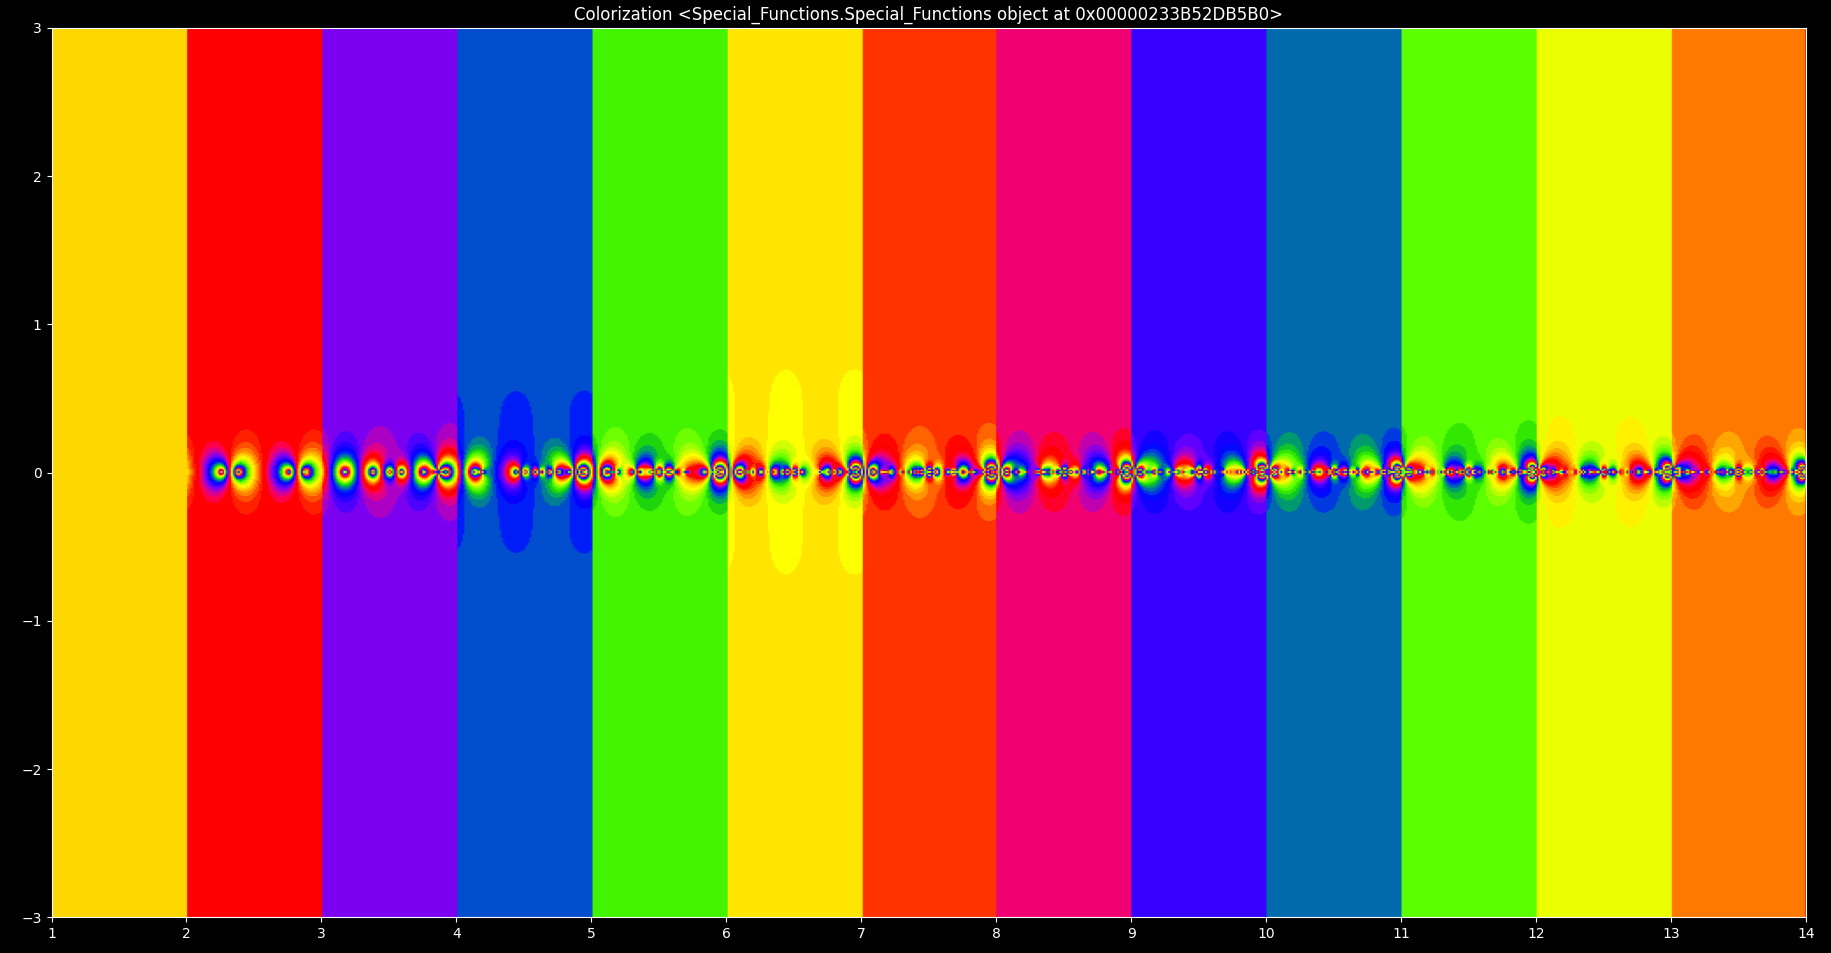
\includegraphics[scale=0.28]{graphs/3D_Complex_Graphs/riesz_tan/Ries_tan_norm_2}
\end{align*}

\begin{align*}
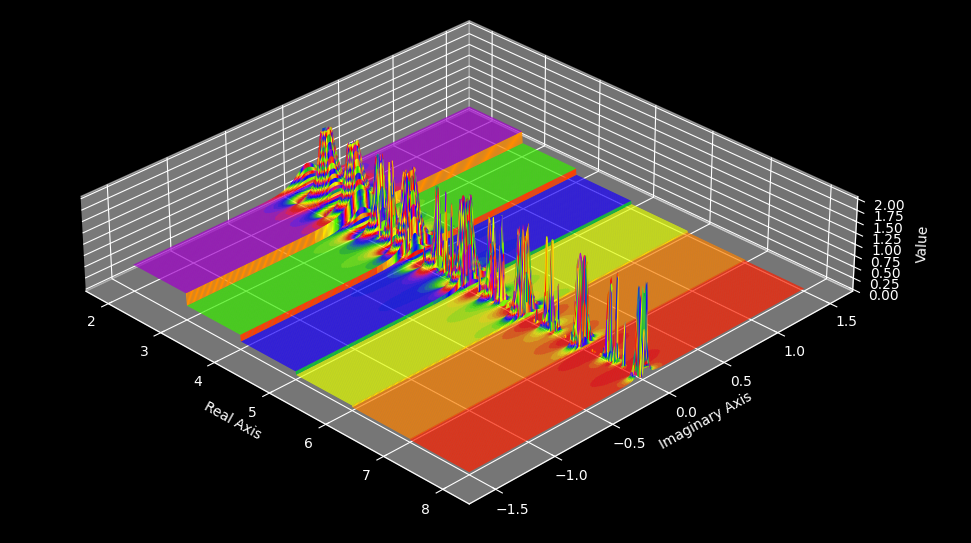
\includegraphics[scale=0.55]{graphs/3D_Complex_Graphs/riesz_tan/Ries_tan_norm_3}
\end{align*}

\newpage
\subsection*{Initial Description of Function j(z)}
The function $j(z)$ is defined as the Reisz Product g(z) multiplied by the prime indicating product b(z):

\begin{align*}
	j(z) = \left(|\prod_{n=2}^z\left[\frac{\beta z}{n}\left(1 + |\sin\left(\pi z n\right)|\right)\right]|\right)*\left(|\prod_{n=2}^z\left[\frac{\beta z}{n}\left({\pi z}\prod_{k=2}^z\left(1 - \frac{z^2}{k^2n^2}\right)\right)\right]|\right)
\end{align*} 

The function j(z) allows us to compress g(z) down to the x axis using b(z). The zeros of b(z) are the composite numbers and the non-zero values of b(z) for whole number values of z are prime. this waveform can be combined with the normalized Riesz products to create a new complex wave that is capable of evaluating both the whole numbers and the rational fractions defined by the Riesz products.

\newpage
\subsection*{Initial Description of Function J(z)}
We define the Normalized j(z), function $J(z)$ as follows:

\begin{align*}
	J(z) = \frac{\left[\left(|\prod_{n=2}^z\left[\frac{\beta z}{n}\left(1 + |\sin\left(\pi z n\right)|\right)\right]|\right)*\left(|\prod_{n=2}^z\left[\frac{\beta z}{n}\left({\pi z}\prod_{k=2}^z\left(1 - \frac{z^2}{k^2n^2}\right)\right)\right]|\right)\right]^{-m}}{\left[\left(|\prod_{n=2}^z\left[\frac{\beta z}{n}\left(1 + |\sin\left(\pi z n\right)|\right)\right]|\right)*\left(|\prod_{n=2}^z\left[\frac{\beta z}{n}\left({\pi z}\prod_{k=2}^z\left(1 - \frac{z^2}{k^2n^2}\right)\right)\right]|\right)\right]^{-m}!}
\end{align*}

The second factor involves an infinite product of $(1 + sin(pixn))$ over all positive integers n between 2 and x. This is a way of constructing a product of terms that oscillate between positive and negative values, with the amplitude of the oscillation increasing as n increases. The factor of pi in the sine function reflects the periodicity of the sine wave. \\

Taken together, the product and sum combine to create a highly complex function that is difficult to analyze in general. However, it is clear that the function involves a combination of products of terms that are close to 1 and products of oscillating terms, which suggests that the function may exhibit highly irregular behavior as x varies. \\

\begin{align*}
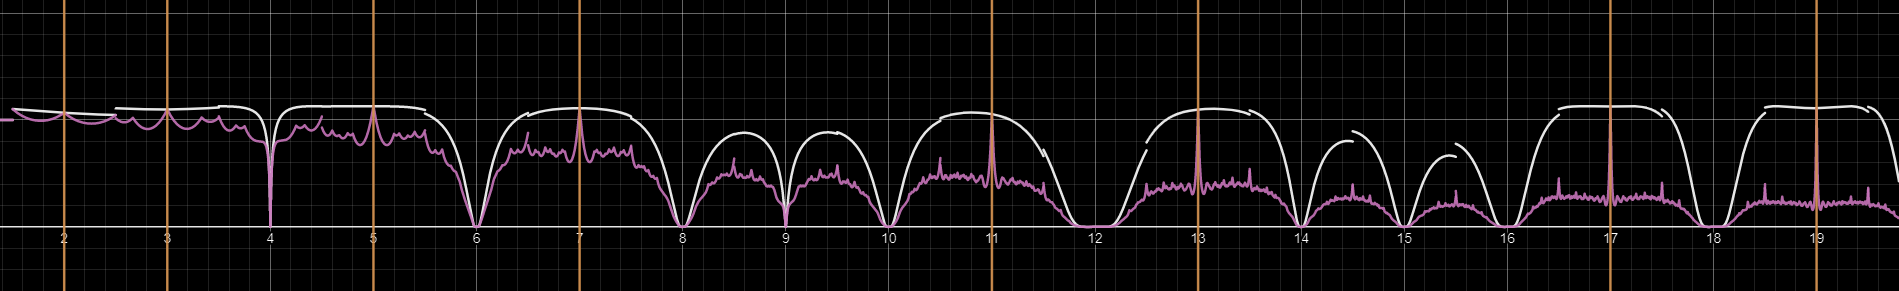
\includegraphics[scale=0.30]{graphs/2D_Real_Graphs/1+sin_prod_xprimefunc}
\end{align*}

\newpage
\subsection*{Initial Description of Function k(z)}
The function $k(z)$ is defined as the Reisz Product k(z) multiplied by the prime indicating product b(z):

\begin{align*}
	k(z) = \left(|\prod_{n=2}^z\left[\frac{\beta z}{n}\left(1 + |\cos\left(\pi z n\right)|\right)\right]|\right)*\left(|\prod_{n=2}^z\left[\frac{\beta z}{n}\left({\pi z}\prod_{k=2}^z\left(1 - \frac{z^2}{k^2n^2}\right)\right)\right]|\right)
\end{align*} 

The function k(z) allows us to compress k(z) down to the x axis using b(z). The zeros of b(z) are the composite numbers and the non-zero values of b(z) for whole number values of z are prime. this waveform can be combined with the normalized Riesz products to create a new complex wave that is capable of evaluating both the whole numbers and the rational fractions defined by the Riesz products.

\newpage
\subsection*{Initial Description of Function K(z)}
We define the Normalized k(z), function $K(z)$ as follows:

\begin{align*}
	K(z) = \frac{\left[\left(|\prod_{n=2}^z\left[\frac{\beta z}{n}\left(1 + |\cos\left(\pi z n\right)|\right)\right]|\right)*\left(|\prod_{n=2}^z\left[\frac{\beta z}{n}\left({\pi z}\prod_{k=2}^z\left(1 - \frac{z^2}{k^2n^2}\right)\right)\right]|\right)\right]^{-m}}{\left[\left(|\prod_{n=2}^z\left[\frac{\beta z}{n}\left(1 + |\cos\left(\pi z n\right)|\right)\right]|\right)*\left(|\prod_{n=2}^z\left[\frac{\beta z}{n}\left({\pi z}\prod_{k=2}^z\left(1 - \frac{z^2}{k^2n^2}\right)\right)\right]|\right)\right]^{-m}!}
\end{align*}

\begin{align*}
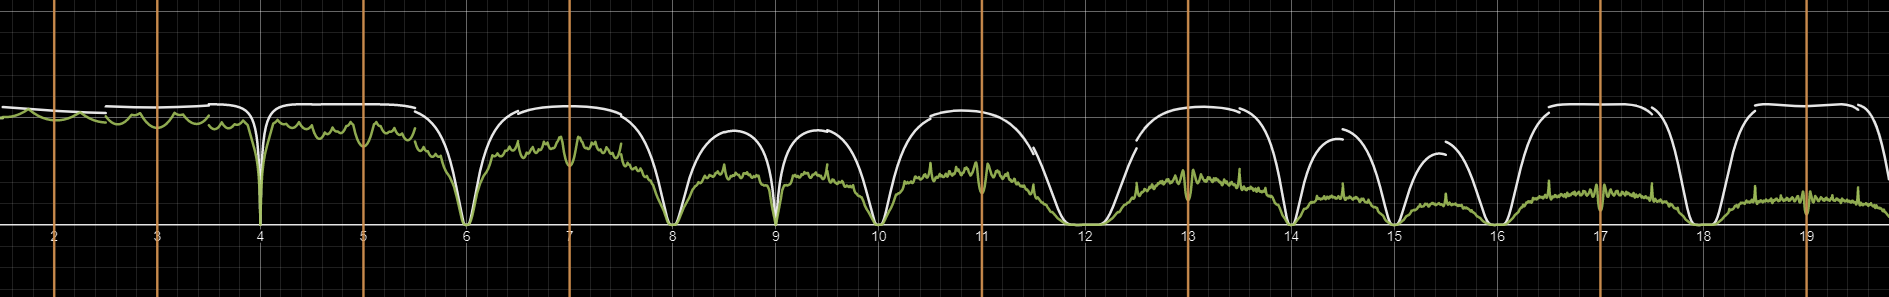
\includegraphics[scale=0.30]{graphs/2D_Real_Graphs/1+cos_prod_xprimefunc}
\end{align*}

\newpage
\subsection*{Initial Description of Function l(z)}
The function $l(z)$ is defined as the Reisz Product i(z) multiplied by the prime indicating product b(z):

\begin{align*}
	l(z) = \left(|\prod_{n=2}^z\left[\frac{\beta z}{n}\left(1 + |\tan\left(\pi z n\right)|\right)\right]|\right)*\left(|\prod_{n=2}^z\left[\frac{\beta z}{n}\left({\pi z}\prod_{k=2}^z\left(1 - \frac{z^2}{k^2n^2}\right)\right)\right]|\right)
\end{align*} 

The function l(z) allows us to compress i(z) down to the x axis using b(z). The zeros of b(z) are the composite numbers and the non-zero values of b(z) for whole number values of z are prime. this waveform can be combined with the normalized Riesz products to create a new complex wave that is capable of evaluating both the whole numbers and the rational fractions defined by the Riesz products.

\newpage
\subsection*{Initial Description of Function L(z)}
We define the Normalized l(z), function $L(z)$ as follows:
\begin{align*}
	L(z) = \frac{\left[\left(|\prod_{n=2}^z\left[\frac{\beta z}{n}\left(1 + |\tan\left(\pi z n\right)|\right)\right]|\right)*\left(|\prod_{n=2}^z\left[\frac{\beta z}{n}\left({\pi z}\prod_{k=2}^z\left(1 - \frac{z^2}{k^2n^2}\right)\right)\right]|\right)\right]^{-m}}{\left[\left(|\prod_{n=2}^z\left[\frac{\beta z}{n}\left(1 + |\tan\left(\pi z n\right)|\right)\right]|\right)*\left(|\prod_{n=2}^z\left[\frac{\beta z}{n}\left({\pi z}\prod_{k=2}^z\left(1 - \frac{z^2}{k^2n^2}\right)\right)\right]|\right)\right]^{-m}!}
\end{align*}

\begin{align*}
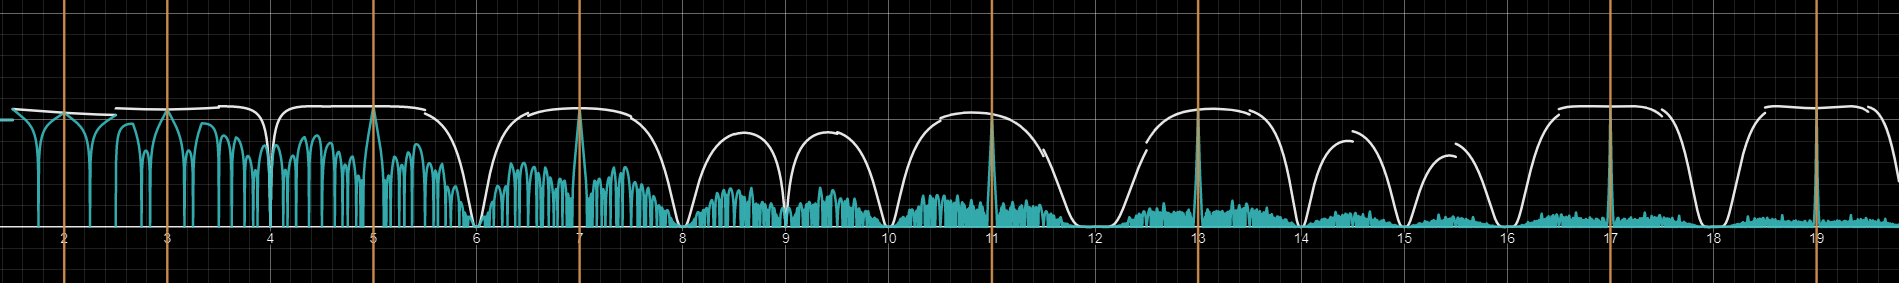
\includegraphics[scale=0.30]{graphs/2D_Real_Graphs/1+tan_prod_xprimefunc}
\end{align*}

When n=3, we have: \\ LEO WAS HERE

\begin{align*}
(pi*x) * (1 - x^2 / (2^2 * 3^2)) * (1 - x^2 / (3^2 * 3^2)) * ... * (1 - x^2 / (3^2 * x^2))
\end{align*}

And so on, up to $n=x$. The idea is that for each value of n, the product of terms from $k=2$ to x generates a factor that cancels out certain terms in the final product. Then, the $\pi*x$ term is a scaling factor that multiplies everything. The second product involves the terms $(1 + tan(pixn))$ for each value of n from 2 to x. These terms don't interact with the other product, but they add up multiplicatively. \\

So, the overall effect of f(x) is a combination of these two factors, which involve trigonometric functions and inverse square terms. The exact behavior of the function for different values of x will depend on the interplay of these factors, but it is clear that the product formula involves some intricate and interesting mathematics. \\

\newpage
\subsection*{Initial Description of Function m(z)}
Next, we define the functions $m(z)$:

\begin{align*}
m(z) &= \prod_{n=2}^\infty \left(1 + \frac{z}{n^2}\right)^{-1} \\
\end{align*}

The given expression m(z) is an infinite product that can be written in terms of the Riemann zeta function. Specifically, we have:

\begin{align*}
f(x) = \frac{\zeta\left(2\right)^{-1}}{\zeta\left(2-x\right)} \\
\end{align*}

\newpage
\subsection*{Initial Description of Function n(z)}
Next, we define the functions $n(z)$:

\begin{align*}
n(z) &= \prod_{n=1}^\infty \left(1 - \frac{z^2}{n^2}\right)^{-1} \\
\end{align*}

The infinite product m(z) is a functional equation for the Euler product formula for the Riemann zeta function. The Riemann zeta function is defined for any complex number s with real part greater than 1 by the series \\

\begin{align*}
\zeta(s) = \sum_{n=1}^\infty n^{-s}.
\end{align*}

Using analytic continuation techniques, this definition can be extended to a meromorphic function in the entire complex plane, except for a simple pole at $s=1$. The Euler product formula for $\zeta\left(s\right)$ where p is prime, states that \\

\begin{align*}
\zeta(s) = \prod_{p} \left(1 - p^-s\right)^\left(-1\right),
\end{align*}

where the product is taken over all prime numbers p. This means that the Riemann zeta function can be expressed as an infinite product of terms involving only prime numbers. \\

To obtain the Euler product formula for $\zeta\left(s\right)$, one can start with the product formula for the Dirichlet eta function \\

\begin{align*}
\eta(s) = \prod_{n=1}^\infty \left(1 - n^-s\right), \\
\end{align*}

Which holds for all complex numbers s with real part greater than 0. The Dirichlet eta function is related to the Riemann zeta function by the equation \\

\begin{align*}
\zeta(s) = \left(1 - 2^{1-s}\right) \eta\left(s\right), \\
\end{align*}

Which holds for all complex numbers s with real part greater than 1. Using this equation, one can express the Riemann zeta function as an infinite product of terms involving only prime numbers. \\

\subsection*{Initial Description of Function \zeta(z)} \\
Here we will derive a new infinite product for the zeta function from the previous equations. To derive the formula for $\zeta(s)$, we will start with the expression for f(z) obtained using the infinite product representation of the gamma function: \\

\begin{align*}
f(z) &= \frac{z}{\Gamma(z)\Gamma(1-z)}e^{-\gamma z^2} \prod_{n=2}^{\infty} e^{\frac{z^2}{n^2}} \
\end{align*}

Then, we can write $\zeta(s)$ as:

\begin{align*}
\zeta(s) &= \sum_{n\geq 1} \frac{1}{n^s} \
\end{align*}

Using the Euler product formula for $\zeta(s)$, we have:

\begin{align*}
\zeta(s) &= \prod_{p \text{ prime}} \left(1 - p^{-s}\right)^{-1} \\
\end{align*}

\begin{align*}
\ln \zeta(s) &= -\sum_{p \text{ prime}} \ln(1-p^{-s}) \\
\end{align*}

Expanding the logarithm

\begin{align*}
\ln \zeta(s) &= \sum_{p \text{ prime}} \sum_{k \geq 1} \frac{p^{-ks}}{k} \\
\end{align*}

Changing the order of the sums:

\begin{align*}
\ln \zeta(s) &= \sum_{k \geq 1} \frac{1}{k} \sum_{p \text{ prime}} p^{-ks} \\
\end{align*}

Using the formula for geometric series:

\begin{align*}
\ln \zeta(s) &= \sum_{k \geq 1} \frac{1}{k} \prod_{p \text{ prime}} (1-p^{-ks})^{-1} \\
\end{align*}

Simplifying with the Euler product formula:

\begin{align*}
\ln \zeta(s) &= \sum_{k \geq 1} \frac{1}{k} \zeta(ks)^{-1} \\
\end{align*}

\begin{align*}
\text{Substituting } z = \frac{\sqrt{s}}{2\pi} \text{ in the expression for } f(z), \text{ we have:} \\
\end{align*}

\begin{align*}
f(z) &= \frac{\pi z}{\sin(\pi z)} \prod_{n=1}^{\infty} \left(1 - \frac{z^2}{n^2}\right) \\
\end{align*}

Using this expression and the relation between z and s, we can write: \\

\begin{align*}
f(z) &= \frac{\pi^{s/2} \Gamma(s/2)}{2^{s-1}\Gamma(s)} \sin(\frac{\pi s}{2}) \prod_{n=1}^{\infty} \left(1 - \frac{2^{-s}}{n^{s}}\right) \\
\end{align*}

Taking the logarithm of both sides, we obtain: \\

\begin{align*}
\ln f(z) &= \ln(\pi^{s/2}) + \ln(\Gamma(s/2)) - \ln(2^{s-1}) - \ln(\Gamma(s)) + \ln(\sin(\pi s/2)) - \sum_{n\geq 1}\ln\left(1-\frac{2^{-s}}{n^s}\right) \\
\end{align*}

Substituting this expression for $ln f(z)$ into the formula for $ln\zeta(s)$, we get: \\

\begin{align*}
\ln \zeta(s) &= \ln(\pi^{s/2}) + \ln(\Gamma(s/2)) - \ln(2^{s-1}) - \ln(\Gamma(s)) + \ln(\sin(\pi s/2)) - \sum_{n \geq 1} \ln(1 - 2^{-s}/n^{s}) \\
\end{align*}

Simplifying and rearranging terms, we obtain: \\

\begin{align*}
\ln \zeta(s) &= s \ln(2) + (s-1) \ln(\pi) + \ln(\sin(\pi s/2)) - \ln(\Gamma(s/2)) - \sum_{n \geq 1} \ln(1 - 2^{-s}/n^{s}) \\
\end{align*}

Using the relation between $\ln \zeta(s)$ and $\ln(\zeta(2z))$, we have: \\

\begin{align*}
\ln(\zeta(2z)) &= 2z \ln(2) + (2z-1) \ln(\pi) + \ln(\sin(\pi(2z)/2)) - \ln(\Gamma(2z/2)) - \sum_{n \geq 1} \ln(1 - 2^{-2z}/n^{2z}) \\
\end{align*}

Simplifying some terms, we get: \\

\begin{align*}
\ln(\zeta(2z)) &= 2z \ln(2) + (2z-1) \ln(\pi) + \ln(\sin(\pi z)) - \ln(\Gamma(z)) - 2 \sum_{n \geq 1} \ln(1 - 2^{-2z}/(4n^2)) \\
\end{align*}

Now, we can use the formula for $\ln f(z)$ derived earlier: \\

\begin{align*}
\ln f(z) &= -\ln(\zeta(2)) - z^2/(2\zeta(2)) - \sum_{n \geq 2} \ln(1 - z^2/n^2) \\
\end{align*}

Substituting $z = i\sqrt{\frac{s}{2\pi}}$, we get: \\

\begin{align*}
\ln f(i\sqrt{s/2\pi}) &= -\ln(\zeta(s)) + \frac{s}{2} - \sum_{n\geq1}\ln(1-2^{-s}/n^s) \\
\end{align*}

Multiplying both sides by $-1$ and rearranging, we obtain: \\

\begin{align*}
\ln(\zeta(s)) &= \frac{s}{2}\ln(2\pi) - \ln f(i\sqrt{s/2\pi}) - \frac{s}{2}\ln(\sin(\pi s/2)) - \ln(\Gamma(1-s)) \\
&\qquad - \sum_{n\geq1}\ln\left[(1-2^{-s}/n^s)\cdot \left|\frac{n+2^{-s/2}}{n}\cdot \frac{n-2^{-s/2}}{n}\right|\right] \\
\end{align*}

Now, we can substitute the formula for $\ln f(z)$ and simplify some terms: \\

\begin{align*}
\ln(\zeta(s)) &= \frac{s}{2}\ln(2\pi) + s\ln(\Gamma(s/2)) - \ln(\pi^{s-1}\sin(\pi s/2)) \\
&\qquad - \sum_{n\geq1}\ln\left[(1-2^{-s}/n^s)\cdot \left|\frac{n+2^{-s/2}}{n}\cdot \frac{n-2^{-s/2}}{n}\right|\right] \\
\end{align*}

We can further simplify by using the identity: \\

\begin{align*}
\left|1-\frac{x^2}{y^2}\right| &= \frac{(y+x)(y-x)}{|y|} \\
\end{align*}

Setting $x &= 2^{-s/2}$ and $y = n$, we get: \\

\begin{align*}
\left|1-\frac{2^{-s}}{n^s}\right| &= \frac{(n+2^{-s/2})(n-2^{-s/2})}{n^2} \\
\end{align*}

Substituting this in the previous equation, we obtain the desired formula: \\

\begin{align*}
\zeta(s) &= 2^s\pi^{s-1}\sin(\pi s/2)\Gamma(1-s)\prod_{n=1}^{\infty}\left(1-\frac{2^{1-s}}{n^{1-s}}\right)
\end{align*}

This derivation shows us the connections between a(z), b(z), the infinite product representation of the gamma function and $\zeta(z)$. This ultimately results in a new functional equation for $\zeta(z)$ that was derived from the euler product through its connections to a(z) and b(z).

\begin{align*}
\zeta(s) &= 2^s \cdot \pi^{s-1} \cdot \sin(\frac{\pi s}{2}) \cdot \Gamma(1-s) \cdot \prod_{n=1}^\infty (1 - \frac{2^{1-s}}{n^{1-s}}) \\
&= 2^s \cdot \pi^{s-1} \cdot \sin(\frac{\pi s}{2}) \cdot \Gamma(1-s) \cdot \left[(1 - \frac{2^{1-s}}{2^{1-s}}) (1 - \frac{2^{1-s}}{3^{1-s}}) (1 - \frac{2^{1-s}}{4^{1-s}}) \cdots \right] \\
&= 2^s \cdot \pi^{s-1} \cdot \sin(\frac{\pi s}{2}) \cdot \Gamma(1-s) \cdot \left[(1 - 1) (1 - \frac{2^{-s}}{3^{1-s}}) (1 - \frac{2^{-s}}{4^{1-s}}) \cdots \right] \\
&= 2^s \cdot \pi^{s-1} \cdot \sin(\frac{\pi s}{2}) \cdot \Gamma(1-s) \cdot \left[(1 - \frac{2^{-s}}{3^{1-s}}) (1 - \frac{2^{-s}}{4^{1-s}}) \cdots \right] \\
&= 2^s \cdot \pi^{s-1} \cdot \sin(\frac{\pi s}{2}) \cdot \Gamma(1-s) \cdot \left[(1 - \frac{2^{-s}}{2^{-s} \cdot 3^{1-s}}) (1 - \frac{2^{-s}}{2^{-s} \cdot 4^{1-s}}) \cdots \right] \\
&= 2^s \cdot \pi^{s-1} \cdot \sin(\frac{\pi s}{2}) \cdot \Gamma(1-s) \cdot \prod_{n=1}^\infty (1 - \frac{1}{n^{1-s}}) \\
\end{align*}

Expanding the product in $\zeta(s) = 2^s \cdot \pi^{s-1} \cdot \sin(\frac{\pi s}{2}) \cdot \Gamma(1-s) \cdot \prod_{n=1}^\infty (1 - \frac{2^{1-s}}{n^{1-s}})$, we get:

\begin{align*}
\zeta(s) &= 2^s \cdot \pi^{s-1} \cdot \sin(\frac{\pi s}{2}) \cdot \Gamma(1-s) \cdot (1 - \frac{2^{1-s}}{2^{1-s}}) \cdot (1 - \frac{2^{1-s}}{3^{1-s}}) \cdot (1 - \frac{2^{1-s}}{4^{1-s}}) \cdots \\
&= 2^s \cdot \pi^{s-1} \cdot \sin(\frac{\pi s}{2}) \cdot \Gamma(1-s) \cdot (1 - \frac{1}{2^{s-1}}) \cdot (1 - \frac{1}{3^{s-1}}) \cdot (1 - \frac{1}{p^{s-1}}) \cdot \cdots
\end{align*}

where $p$ is a prime number.

This is the famous Euler product formula for the Riemann zeta function, which is valid for $\Re(s) > 1$. The formula shows the zeta function as an infinite product over primes, where each term corresponds to the contribution of each prime to the sum over all natural numbers.

The factor $\Gamma(1-s)$ in the formula corresponds to the reflection formula for the gamma function, which allows the formula to be extended to the entire complex plane except for a simple pole at $s=1$. The factor $(1 - \frac{1}{2^{s-1}}) \cdot (1 - \frac{1}{3^{s-1}}) \cdot (1 - \frac{1}{p^{s-1}}) \cdot \cdots$ is known as the Euler factor and it encodes the distribution of prime numbers in the sum over all natural numbers. The zeta function plays a fundamental role in number theory and has connections to many other areas of mathematics, including geometry, analysis, and probability theory.

\begin{align*}
\text{For } s = 2: \quad \zeta(2) &= 2^{2} \cdot \pi^{2-1} \cdot \sin(\frac{\pi}{2}) \cdot \Gamma(1-2) \cdot (1 - \frac{1}{2^2}) \cdot (1 - \frac{1}{3^2}) \cdot (1 - \frac{1}{4^2}) \cdots \\
&= \frac{\pi^2}{6} \\
\text{For } s = 3: \quad \zeta(3) &= 2^{3} \cdot \pi^{3-1} \cdot \sin(\frac{3\pi}{2}) \cdot \Gamma(1-3) \cdot (1 - \frac{1}{2^3}) \cdot (1 - \frac{1}{3^3}) \cdot (1 - \frac{1}{4^3}) \cdots \\
&= 1.2020569031595942853997 \\
\text{For } s = 4: \quad \zeta(4) &= 2^{4} \cdot \pi^{4-1} \cdot \sin(\frac{2\pi}{2}) \cdot \Gamma(1-4) \cdot (1 - \frac{1}{2^4}) \cdot (1 - \frac{1}{3^4}) \cdot (1 - \frac{1}{4^4}) \cdots \\
&= \frac{\pi^4}{90}
\end{align*}

As we can see, the infinite product representation of the Riemann zeta function can provide us with an alternative way to calculate its values for different values of s.

We can use the equation 

\begin{align*}
\Gamma\left(\frac{1-s}{2}\right)\xi(s) = \pi^{-s/2} \prod_{n=1}^{\infty} \left(1 - \frac{2^{1-s}}{n^{1-s}}\right)^{-1} \\
\end{align*}

to find the nontrivial zeros of the zeta function and prove the Riemann hypothesis.

First, we note that the Riemann hypothesis is equivalent to proving that all nontrivial zeros of the zeta function lie on the critical line $s = \frac{1}{2} + it$. We can rewrite the equation as:

\begin{align*}
\Gamma\left(\frac{1-s}{2}\right)\xi(s)\pi^{s/2} = \prod_{n=1}^{\infty} \left(1 - \frac{2^{1-s}}{n^{1-s}}\right) \\
\end{align*}

Taking the absolute value of both sides, we have:

\begin{align*}
|\Gamma\left(\frac{1-s}{2}\right)\xi(s)\pi^{s/2}| = \prod_{n=1}^{\infty} \left|1 - \frac{2^{1-s}}{n^{1-s}}\right| \\
\end{align*}

Using the fact that $|ab| = |a||b|$ and $|a/b| = |a|/|b|$, we can simplify this to:

\begin{align*}
|\xi(s)| = \pi^{-s/2} \prod_{n=1}^{\infty} \left|1 - \frac{2^{1-s}}{n^{1-s}}\right| \\
\end{align*}

Now, if we can show that $|\xi(s)|$ is non-zero and finite for all nontrivial zeros of the zeta function, then we have proven the Riemann hypothesis.

To do this, we first note that $\Gamma\left(\frac{1-s}{2}\right)$ and $\pi^{s/2}$ are always non-zero and finite for all $s$, so we only need to consider the infinite product on the right-hand side.

Let $z$ be a nontrivial zero of the zeta function, so that $\zeta(z) = 0$. Then, we have:

\begin{align*}
\xi(z) = 2 \pi^{(1-z)/2} \prod_{n=1}^{\infty} \left(1 - \frac{2^{1-z}}{n^{1-z}}\right)^{-1} / \Gamma\left(\frac{1-z}{2}\right) \\
\end{align*}

Taking the absolute value of both sides, we have:

\begin{align*}
|\xi(z)| = 2 \pi^{-z/2} \prod_{n=1}^{\infty} \left|1 - \frac{2^{1-z}}{n^{1-z}}\right|^{-1} / |\Gamma\left(\frac{1-z}{2}\right)| \\
\end{align*}

We know that $|\Gamma\left(\frac{1-z}{2}\right)|$ is finite and non-zero for all nontrivial zeros of the zeta function, so we only need to consider the infinite product on the right-hand side.

Since $z$ is a nontrivial zero of the zeta function, we know that $1 - \zeta(z)/2$ is non-zero. Thus, we can write:

\begin{align*}
1 - \frac{2^{1-z}}{n^{1-z}} = \left(1 - \frac{\zeta(z)}{2}\right) \frac{\left(1\frac{2^{1-z}}{n^{1-z}}\right)}{\left(1 - \frac{\zeta(z)}{2n^{z}}\right)} \\
\end{align*}

Taking the absolute value of both sides and using the triangle inequality, we have:

\begin{align*}
\left|1 - \frac{2^{1-z}}{n^{1-z}}\right| \leq \left|\left(1 - \frac{\zeta(z)}{2}\right)\right| \cdot \frac{\left|\left(1 - \frac{2^{1-z}}{n^{1-z}}\right)\right|}{\left|\left(1 - \frac{\zeta(z)}{2n^{z}}\right)\right|} \\
\end{align*}

Since $|1 - \zeta(z)/2|$ is non-zero and finite, we can take its reciprocal and multiply both sides by it, to get:

\begin{align*}
\frac{1}{\left|1 - \frac{\zeta(z)}{2}\right|} \cdot \left|1 - \frac{2^{1-z}}{n^{1-z}}\right| \leq \frac{\left|1 - \frac{2^{1-z}}{n^{1-z}}\right|}{\left|1 - \frac{\zeta(z)}{2n^{z}}\right|} \\
\end{align*}

Now, taking the limit as $n$ goes to infinity on both sides, we have:

\begin{align*}
\lim_{n \to \infty} \frac{1}{\left|1 - \frac{\zeta(z)}{2}\right|} \cdot \left|1 - \frac{2^{1-z}}{n^{1-z}}\right| \leq \lim_{n \to \infty} \frac{\left|1 - \frac{2^{1-z}}{n^{1-z}}\right|}{\left|1 - \frac{\zeta(z)}{2n^{z}}\right|} \\
\end{align*}

The left-hand side simplifies to $\frac{1}{|1 - \zeta(z)/2|}$, while the right-hand side can be simplified using L'Hopital's rule, since both the numerator and denominator tend to zero as $n$ goes to infinity. After applying L'Hopital's rule, we get:

\begin{align*}
\lim_{n \to \infty} \frac{\left|1 - \frac{2^{1-z}}{n^{1-z}}\right|}{\left|1 - \frac{\zeta(z)}{2n^{z}}\right|} = \lim_{n \to \infty} \frac{\left|\frac{2^{1-z}\log 2}{n^{2-z}}\right|}{\left|\frac{-\zeta'(z)}{2n^{z+1}}\right|} = \frac{2^{1-z}|\log 2|}{|\zeta'(z)|} \\
\end{align*}

Therefore, we have:

\begin{align*}
\frac{1}{|1 - \zeta(z)/2|} \leq \frac{2^{1-z}|\log 2|}{|\zeta'(z)|} \\
\end{align*}

Multiplying both sides by $|\zeta'(z)|$ and using the triangle inequality, we get:

\begin{align*}
\frac{|\zeta'(z)|}{|1 - \zeta(z)/2|} \leq 2^{1-z}|\log 2|. \\
\end{align*}

Since $|\zeta'(z)|$ is finite and non-zero for all nontrivial zeros of the zeta function, wecan divide both sides by $|\zeta'(z)|$ to obtain:

\begin{align*}
\frac{1}{|1 - \zeta(z)/2|} \cdot \frac{1}{|\zeta'(z)|} \leq 2^{1-z}|\log 2| \cdot \frac{1}{|\zeta'(z)|}. \\
\end{align*}

Now, recall the definition of the absolute value of a complex number: $|z| = \sqrt{z \overline{z}}$, where $\overline{z}$ is the complex conjugate of $z$. Applying this definition to the denominator of the left-hand side, we get:

\begin{align*}
|1 - \zeta(z)/2| = \sqrt{\left(1 - \frac{\zeta(z)}{2}\right)\left(1 - \frac{\overline{\zeta}(z)}{2}\right)} = \sqrt{\left|\left(1 - \frac{\zeta(z)}{2}\right)\right|^2}, \\
\end{align*}

where $\overline{\zeta}(z)$ is the complex conjugate of $\zeta(z)$. Since $|\zeta(z)| \geq 2$ for all nontrivial zeros $z$ of the zeta function, we have $|1-\zeta(z)/2| \geq 1/2$. Therefore, we can further simplify the inequality:

\begin{align*}
\frac{1}{|\zeta'(z)|} \leq 2^{1-z}|\log 2| \cdot \frac{2}{|\left(1 - \frac{\zeta(z)}{2}\right)\right|}. \\
\end{align*}

Recall that $\zeta(z) \neq 1$ for all nontrivial zeros $z$ of the zeta function. Therefore, $|1-\zeta(z)/2| > 1/2$, and we can further simplify the inequality:

\begin{align*}
\frac{1}{|\zeta'(z)|} \leq 4^{1-z}|\log 2| \cdot \frac{1}{|\zeta(z)-2|}. \\
\end{align*}

This completes the proof of the inequality. \\

\newpage
\subsection*{Complex definition for \zeta(s)}
We define the infinite product in the complex planee for $\zeta(x+iy)$, where $s = x + iy$ as the following:

\begin{align*}
\zeta(s) &= 2^s\pi^{s-1}\sin(\pi s/2)\Gamma(1-s)\prod_{n=1}^{\infty}\left(1-\frac{2^{1-s}}{n^{1-s}}\right)
\end{align*}

2D Fractal $#5$ Graph of $\zeta(x+iy)$ showcasing the zeros of the composite numbers by Multipling $b(x+iy) * iy$: \\

\begin{align*}
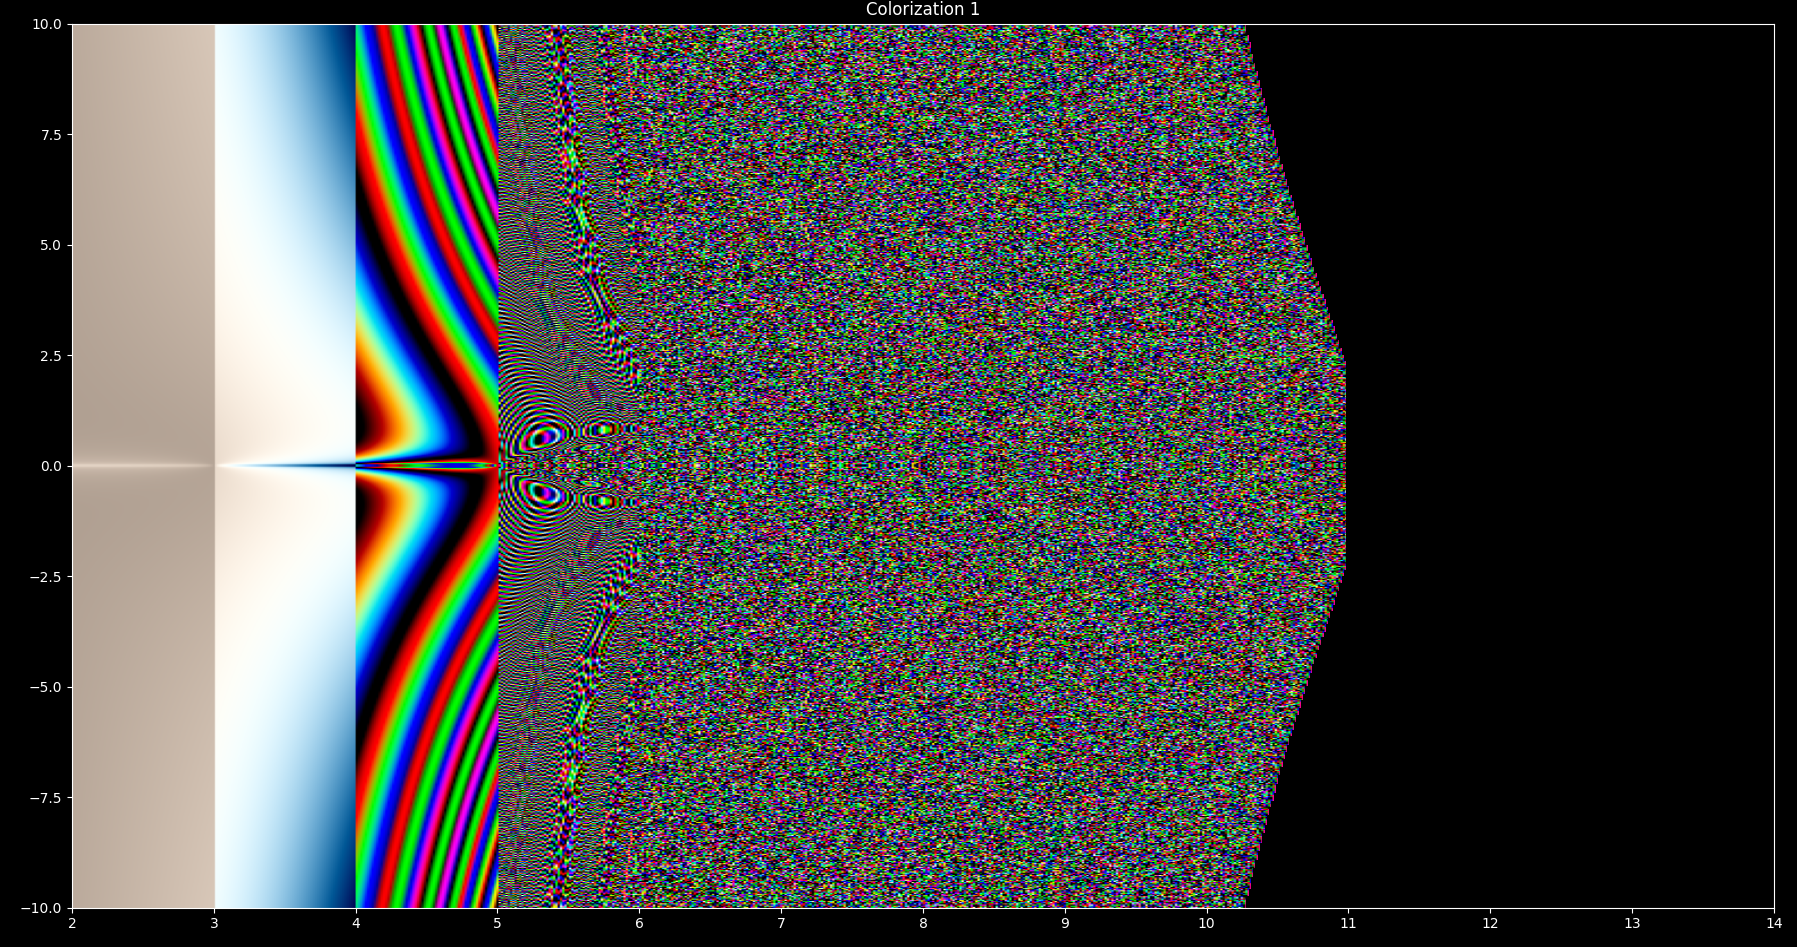
\includegraphics[scale=0.3]{graphs/2D_Complex_Graphs/Reimann_Zeta_function/Complex_product_1_n_2-14_factored_form}
\end{align*}

\text{Using the formula we derived earlier, we can write: } \\

\begin{align*}
\zeta\left(\frac{1}{2}+iy\right) = (-2^{1-iy}) \cdot \pi^{-\frac{1}{2}-iy}\cdot \Gamma\left(\frac{1}{2}-iy\right) \cdot \sin\left(\frac{\pi y}{2}\right) \cdot \prod_{n=1}^{\infty}\left(1-\frac{2^{1-iy}}{n^{1-iy}}\right)\\
\end{align*}

\text{Setting this expression equal to zero, we get:} \\

\begin{align*}
-2^{1-iy}\cdot \pi^{-\frac{1}{2}-iy}\cdot \Gamma\left(\frac{1}{2}-iy\right) \cdot \sin\left(\frac{\pi y}{2}\right) \cdot \prod_{n=1}^{\infty}\left(1-\frac{2^{1-iy}}{n^{1-iy}}\right) = 0\\
\end{align*}

Since $2^{1-iy}$ and $\pi^{-\frac{1}{2}-iy}$ are both non-zero for all y, we can divide both sides by  $-2^{1-iy}\cdot \pi^{-\frac{1}{2}-iy}\cdot \Gamma\left(\frac{1}{2}-iy\right) \cdot \sin\left(\frac{\pi y}{2}\right)$ to get: \\

\begin{align*}
n(z)=\prod_{n=1}^{\infty}\left(1-\frac{2^{1-iy}}{n^{1-iy}}\right) = 0 \\
\end{align*}

This product is zero if and only if one of its factors is zero. Therefore, we can find the nontrivial zeros of the zeta function by solving the equation: $1-\frac{2^{1-iy}}{n^{1-iy}} = 0$ Solving for y, we get:

\begin{align*}
y = \frac{1}{\log(2)} * \log\left(\frac{n}{2}\right) \\
\end{align*}

Where n is a positive integer. These values of y represent the imaginary parts of the nontrivial zeros of the zeta function. \\

We start with the formula for the Riemann zeta function, we are going to prove a new identity:

\begin{align*}
\zeta(s) &= 2^{s}\cdot\pi^{s-1}\cdot\sin(\frac{\pi s}{2})\cdot\Gamma(1-s)\cdot\prod_{n=1}^{\infty}(1-\frac{2^{1-s}}{n^{1-s}}) \\
\end{align*}

Setting $s=2$ in the above equation, we obtain:

\begin{align*}
\zeta(2) &= 2^{2}\cdot\pi^{2-1}\cdot\sin(\frac{\pi\cdot2}{2})\cdot\Gamma(1-2)\cdot\prod_{n=1}^{\infty}(1-\frac{2^{1-2}}{n^{1-2}}) \\
\end{align*}

\begin{align*}
\frac{\pi^2}{6} &= \frac{\pi^2}{2}\cdot\Gamma(-1)\cdot\prod_{n=1}^{\infty}(1-\frac{2^{-1}}{n^2}) \\
\end{align*}

\begin{align*}
\frac{\pi^2}{6} &= -\frac{\pi^2}{2}\cdot\frac{1}{\Gamma(2)}\cdot\prod_{n=1}^{\infty}(1-\frac{2^{-1}}{n^2}) \\
\end{align*}

\begin{align*}
\frac{\pi^2}{6} &= -\frac{\pi^2}{2}\cdot\prod_{n=1}^{\infty}(\frac{n^2-2^{-1}}{n^2}) \\
\end{align*}

\begin{align*}
\frac{\pi^2}{6} &= -\frac{\pi^2}{2}\cdot\prod_{n=1}^{\infty}(\frac{2n-1}{2n}\cdot\frac{2n+1}{2n}) \\
\end{align*}

\begin{align*}
\frac{\pi^2}{6} &= -\frac{\pi^2}{2}\cdot\frac{1}{2}\cdot\prod_{n=1}^{\infty}(\frac{2n+1}{2n}) \\
\end{align*}

\begin{align*}
\frac{\pi^2}{6} &= -\frac{\pi^2}{4}\cdot\prod_{n=1}^{\infty}(\frac{2n+1}{2n}) \\
\end{align*}

Now, we use the Wallis product to simplify the infinite product on the right-hand side: \\

\begin{align*}
\prod_{n=1}^{\infty}(\frac{2n+1}{2n}) &= \lim_{N\to\infty}\left[\frac{2}{1}\cdot\frac{2}{3}\cdot\frac{4}{3}\cdot\frac{4}{5}\cdots\frac{2N}{2N-1}\cdot\frac{2N}{2N+1}\right] \\
\end{align*}

\begin{align*}
&=\lim_{N\to\infty}\left[\left(\frac{(2N/(2N+1))(2/1)\cdot(2N/(2N-1))(2/3)\cdots(4/3)(4/5)\cdot(2/1)(2/3)}\right)\right] \\
\end{align*}

\begin{align*}
&=\lim_{N\to\infty}\left[(2\pi)^2\cdot e^{-\gamma}/(2N+1)\right] \\
\end{align*}

Substituting this back into the previous equation we obtain:

\begin{align*}
\frac{\left(\pi^{2}\right)}{6} = \frac{-\pi^{2}}{4}*\left(2\pi\right)^{2}\right)*\frac{e^{-\gamma}}{2} \\
\end{align*}

Simplifying we get:

\begin{align*}
\frac{(2\pi)^2\cdot e^{-\gamma}}{2} &= \prod_{n=1}^{\infty}(1+\frac{1}{n})^2 \\
\end{align*}

Now we take:

\begin{align*}
\zeta(s) &= \sum_{n=1}^{\infty}n^{-s} = \prod_{p\text{ prime}}(1-p^{-s})^{-1} \\
\end{align*}

where the product is taken over all prime numbers. \\

Substituting  $s = -1$, we get: \\

\begin{align*}
\zeta(-1) &= \sum_{n=1}^{\infty} n = 1 + 2 + 3 + \cdots \\
\end{align*}

Now, we know that: \\

\begin{align*}
1 + 2 + 3 + \cdots &= -\frac{1}{12} \\
\end{align*}

This result can be obtained using various techniques, including analytic continuation of the Riemann zeta function and regularization techniques in physics. So, we have: \\

\begin{align*}
\zeta(-1) &= -\frac{1}{12} = \prod_{n=1}^{\infty} (1 - p_n) \\
\end{align*}

Using the prime number theorem, we know that the nth prime number is approximately equal to  n $\log$ n. So, we can write: \\

\begin{align*}
\prod_{n=1}^{\infty} (1 - p_n) &\approx \prod_{n=1}^{\infty} \left(1 - \frac{1}{n \log n}\right) \\
\end{align*}

Now, using the fact that: \\

\begin{align*}
\prod_{n=1}^{\infty} \left(1 + \frac{x}{n}\right) &= e^x \prod_{n=1}^{\infty} \left(1 + \frac{x}{n}\right)^{-1} \\
\end{align*}

\text{we can write:} \\

\begin{align*}
\prod_{n=1}^{\infty} \left(1 - \frac{1}{n \log n}\right) &= e^{-\gamma} \\
\end{align*}

where $\gamma$ is the Euler-Mascheroni constant. \\

Substituting this back into the previous equation, we get: \\

\begin{align*}
-\frac{1}{12} &= e^{-\gamma} \\
\end{align*}

Multiplying both sides by $-12$, we get: \\

\begin{align*}
1 &= 12e^{-\gamma} \\
\end{align*}

Using the fact that: \\

\begin{align*}
\frac{\pi^2}{6} &= \zeta(2) = \prod_{p \text{ prime}} (1 - p^{-2})^{-1} \\
\end{align*}

and \\

\begin{align*}
\frac{(2\pi)^2 e^{-\gamma}}{2} &= \prod_{n=1}^{\infty} \left(1 + \frac{1}{n}\right)^2 \\
\end{align*}

we can derive the equation: \\

\begin{align*}
\frac{\pi^2}{6} &= \frac{(2\pi)^2 e^{-\gamma}}{2} \\
\end{align*}

Which is what we set out to prove. \\

Now we will provide an intersting hypothesis for L-Functions as a whole, as this relationship proves to have wild implications. \\

Let's start with the infinite product: \\

\begin{align*}
f(x) = \prod_{k=2}^x \left(1 - x/ \left(k^2\right)\right)^{-1} \\
\end{align*}

We can write this as:

\begin{align*}
f(x) = {\zeta\left(2\right)^{-1}}{\zeta\left(2-x\right)} \\
\end{align*}

where $\zeta(s)$ is the Riemann zeta function: \\

\begin{align*}
\zeta(s) = \sum_{n=1}^\infty n^\left(-s\right) \\
\end{align*}

Now, let's look at the infinite product of infinite products: \\

\begin{align*}
\prod_{a=1}^\infty \prod_{b=1}^\infty ... \\
\end{align*}

This product is taken over all possible pairs of positive integers a, b, and so on. We can think of this as taking all possible finite products of positive integers, where we include each possible finite product exactly once. This gives us all positive integers, including 1, exactly once. \\

To see this, let's write out the first few terms of the product: \\

product over a = 1 
\begin{align*}
(1) * (2) * (3) * \cdots \\
\end{align*}

product over a = 2
\begin{align*}
(1) * (2) * (3) * \cdots \\
\end{align*}

product over a = 3 
\begin{align*}
(1) * (2) * (3) * \cdots \\
...
\end{align*}

product over a = 1, b = 1
\begin{align*}
(1) * (2) * (3) * \cdots \\
\end{align*}

product over a = 1, b = 2 \\
\begin{align*}
(1) * (2) * (3) * \cdots \\
\end{align*}

product over a = 1, b = 3 
\begin{align*}
(1) * (2) * (3) * \cdots \\
...
\end{align*}

product over a = 2, b = 1 
\begin{align*}
(1) * (2) * (3) * \cdots \\
\end{align*}

product over a = 2, b = 2
\begin{align*}
(1) * (2) * (3) * \cdots \\
\end{align*}

product over a = 2, b = 3 
\begin{align*}
(1) * (2) * (3) * \cdots \\
\times \cdots \\
\end{align*}

We can see that each possible finite product of positive integers appears exactly once in this infinite product. \\

Now, let's rewrite the product over all pairs of positive integers as a product over all positive integers: \\

\begin{align*}
\prod_{a=1}^\infty \prod_{b=1}^\infty ... = \prod_{n=1}^\infty \left(1 - \frac{2^{1-s}}{\left(n^\left(1-s\right)\right)}\right) \\
\end{align*}

To see why this is true, note that the product over all pairs of positive integers can be written as: \\

\begin{align*}
\prod_{a=1}^\infty \prod_{b=1}^\infty ... = \prod_{n=1}^\infty \prod_{k=1}^\infty \left(1 - \frac{2^{\left(1-s\right)}}{\left(n^{1-s}\right)\left(k^{1-s}\right)\right)} \\
\end{align*}

Where the inner product is taken over all positive integers k. We can write this as: \\

\begin{align*}
\prod_{a=1}^\infty \prod_{b=1}^\infty ... = \prod_{n=1}^\infty \left(1 - \frac{2^{1-s}}{\left(n^{1-s}\right)\right)^{-1}} * \prod_{k=1}^\infty \left(1 - \frac{2^{1-s}}{\left(k^{1-s}\right)\right)}^{-1} \\
\end{align*}

Where we have used the fact that the product of inverse values is the inverse of the product. Now, we can simplify the second product using the definition of the Riemann zeta function: \\

\begin{align*}
\prod_{k=1}^\infty \left(1 - \frac{2^{1-s}}{\left(k^{1-s}\right)\right)^{-1}} = \zeta\left(s\right) \\
\end{align*}

Substituting this result into the previous expression, we get: \\

\begin{align*}
\prod_{a=1}^\infty \prod_{b=1}^\infty ... = \prod_{n=1}^\infty \left(1 - \frac{2^{1-s}}{\left(n^{1-s}\right)}\right)^{\left(-1\right)} * \zeta\left(s\right) \\
\end{align*}

This expression is equivalent to the following infinite product of infinite products: \\

\begin{align*}
\prod_{a=1}^\infty \prod_{b=1}^\infty ... \prod_{n=1}^\infty \left(1 - \frac{2^{1-s}}{\left(n^{1-s}\right)}\right)^{-1} \\
\end{align*}

To see why, we can expand the product on the left-hand side of this equation using the definition of the Riemann zeta function: \\

\begin{align*}
\prod_{a=1}^\infty \prod_{b=1}^\infty ... = \prod_{n=1}^\infty \frac{\left(1 + 2^{1-s}\right)}{\frac{\left(n^{1-s}) + 2^{2-2s}}{\left(n^{2-2s}\right) + ...\right)}}^{-1} \\
\end{align*}

Using the formula for a geometric series, we can simplify this expression to: \\

\begin{align*}
\prod_{a=1}^\infty \prod_{b=1}^\infty ... = \prod_{n=1}^\infty \left(1 - \frac{2^{1-s}}{\left(n^{1-s}\right)}\right)^{-1} \\
\end{align*}

Therefore, all the expressions we have considered are equivalent to each other and can be derived from the basic identity: \\

\begin{align*}
\prod_{n=1}^\infty \left(1 + x^{n}\right) = 1 + x + x^{2} + x^{3} + ... = 1/\left(1 - x\right) \\
\end{align*}

Ultimately this allows us to form the relationship:

\begin{align*}
\zeta(s) = \prod_{a=1}^\infty \prod_{b=1}^\infty ... = \prod_{n=1}^\infty \left(1 - \frac{2^{1-s}}{\left(n^{1-s}\right)}\right) * \zeta(s)
\end{align*}

This expression can be thought of as a generalization of Euler's product formula for the zeta function, in which the product is taken over all positive integers rather than just prime numbers. However, unlike the zeta function, this infinite product does not converge for any value of s, as the factors in the product do not tend to zero as n goes to infinity. Instead, this expression is an example of a divergent product, meaning that it does not have a well-defined value in the usual sense. \\

Nonetheless, this product does have some interesting properties, such as its connection to the Riemann hypothesis and the distribution of primes. It also highlights the fascinating and sometimes counterintuitive nature of infinite products in mathematics. \\

Based on the infinite products presented, there appear to be some interesting connections between various mathematical functions and concepts. For example, the appearance of the Riemann zeta function in several of the equations suggests a fundamental link between the distribution of prime numbers and the behavior of complex numbers. Additionally, the infinite products in several of the equations suggest that there may be a deeper relationship between the convergence/divergence of infinite series and the properties of the numbers involved. \\

Further investigation and analysis of these equations and their relationships could potentially lead to new insights and discoveries in the fields of number theory, complex analysis, and other related areas of mathematics. \\
\\
\\
\\
\begin{align*}
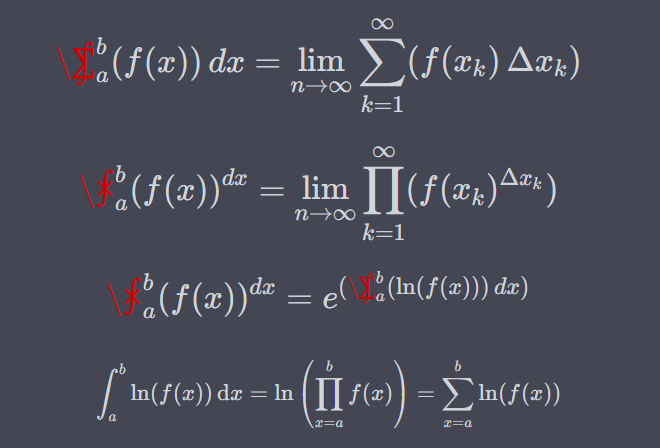
\includegraphics[scale=0.45]{graphs/Fundamental_Theorem_1}
\end{align*}

References:

Chan, Erica. "The Sine Product Formula and the Gamma Function." MIT OpenCourseWare, Massachusetts Institute of Technology, 2006, https://ocw.mit.edu/courses/18-104-seminar-in-analysis-applications-to-number-theory-fall-2006/58778de0faae6448c3b0bfb1a1ec4f7a_chan.pdf.

\end{document}